\documentclass[12pt]{article}

\usepackage[top=2cm,bottom=3cm,left=3cm,right=2cm]{geometry}
\usepackage{amsmath}


\DeclareMathOperator*{\argmax}{argmax}
\DeclareMathOperator*{\argmin}{argmin}
\DeclareMathOperator*{\E}{\mathbb{E}}

\usepackage{hyperref}

\usepackage{booktabs}
\usepackage{caption}
\usepackage{amsfonts}
\usepackage{amsthm}
\usepackage{fontspec}
\usepackage{hyperref}
\usepackage[thinc]{esdiff}
\usepackage{cite}
\usepackage{pdfpages}
\usepackage{graphicx}
\hypersetup{
    colorlinks=true,
    linkcolor=blue,
    filecolor=magenta,      
    urlcolor=cyan,
    citecolor=cyan
}


% this package for increase or decrease vertical space between section chapter paragraph etc.
\usepackage{titlesec}

%tikz package for drawing graphs%
\usepackage{tkz-berge}
\usepackage{tikz}

\usetikzlibrary{arrows}

\usetikzlibrary{decorations.markings}
\usetikzlibrary{positioning,chains,fit,shapes,calc}

\usetikzlibrary{trees,positioning,fit,arrows,decorations.pathreplacing}

\usetikzlibrary{shapes.geometric, shapes.misc, positioning, calc, arrows.meta}
\renewcommand{\figurename}{Նկ.}
% the figure insert specific place with [H] param
\usepackage{float}




\newcommand{\undertextline}[2]{ {
\renewcommand{\arraystretch}{0.7}
\begin{tabular}{p{#2cm}}
\\
\hline
\centering{{\fontsize{8pt}{8pt} \textit{#1}}}
\end{tabular}} }


\newcommand*{\vertbar}{\rule[-1ex]{0.5pt}{2.5ex}}
\newcommand*{\horzbar}{\rule[.5ex]{2.5ex}{0.5pt}}




% increase distance between two lines%
\renewcommand{\baselinestretch}{1.5}

% increase vertical space between section subsection%
\titlespacing{\section}
{0pt}{5ex plus 1ex minus .2ex}{3ex plus .2ex}
\titlespacing{\subsection}
{0pt}{5ex plus 1ex minus .2ex}{3ex plus .2ex}


\setmainfont[Path = fonts/,
BoldItalicFont=arnamu_italic_bold.ttf,
BoldFont      =arnamu_bold.ttf,
ItalicFont    =arnamu_italic.ttf]{arnamu.ttf}

\renewcommand{\contentsname}{Բովանդակություն}
\renewcommand{\refname}{Գրականություն}

\renewcommand{\tablename}{Աղյուսակ}
%\usepackage{mathtools}
%\newcommand\defeq{\stackrel{\mathclap{\normalfont\mbox{def}}}{=}}
\newcommand\defeq{\mathrel{\overset{\makebox[0pt]{\mbox{\normalfont\tiny\sffamily def}}}{=}}}

\sloppy
\begin{document}

\newtheorem{theorem}{Թեորեմ}
\newtheorem{lemma}{Լեմմա}
\newtheorem{corollary}{Հետևանք}
\newtheorem{preposition}{Պնդում}
\newtheorem{defination}{Սահմանում}
\newtheorem{remark}{Դիտողություն}
\newtheorem*{remark*}{Դիտողություն}


\theoremstyle{definition} %After this line new defined commands by \newthorem will be non italic.%
\newtheorem{innercustomcase}{Դեպք}
\newenvironment{customcase}[1]
  {\renewcommand\theinnercustomcase{#1}\innercustomcase}
  {\endinnercustomcase}
\newtheorem{case}{Դեպք}

\raggedbottom


\begin{titlepage}

\begin{center}
{\fontsize{18pt}{18pt} \selectfont \textbf{ԵՐԵՎԱՆԻ ՊԵՏԱԿԱՆ ՀԱՄԱԼՍԱՐԱՆ\\}} 
\vspace{7mm}
{\fontsize{18pt}{18pt} \selectfont \textbf{ԻՆՖՈՐՄԱՏԻԿԱՅԻ ԵՎ ԿԻՐԱՌԱԿԱՆ ՄԱԹԵՄԱՏԻԿԱՅԻ ՖԱԿՈՒԼՏԵՏ\\}}
\vspace{7mm}
{\fontsize{16pt}{16pt} \selectfont \textbf{ Թվային անալիզի և մաթեմատիկական մոդելավորման ամբիոն\\}}
\vspace{7mm}
{\fontsize{18pt}{18pt} \selectfont \textbf{ «ԹՎԱՅԻՆ ԱՆԱԼԻԶ ԵՎ ՄԱԹԵՄԱՏԻԿԱԿԱՆ ՄՈԴԵԼԱՎՈՐՈՒՄ»
ԿՐԹԱԿԱՆ ԾՐԱԳԻՐ\\}}

\vspace{25mm}
{\fontsize{18pt}{18pt} \selectfont \textbf{ՄԻՆԱՍՅԱՆ ԳԵՎՈՐԳ ՄԱՆՎԵԼԻ\\}}
\vspace{15mm}
{\fontsize{18pt}{18pt} \selectfont \textbf{ՄԱԳԻՍՏՐՈՍԱԿԱՆ ԹԵԶ\\}}
\vspace{5mm}
{\fontsize{16pt}{16pt} \selectfont \textbf{ՏՐԱՆՍՖԵՐԱՅԻՆ ՈՒՍՈՒՑՄԱՆ ՈՐՈՇԱԿԻ ՄԵԹՈԴԻ ԸՆԴՀԱՆՐԱՑՄԱՆ ՍԽԱԼԱՆՔԻ ԳՆԱՀԱՏՄԱՆ ՄԱՍԻՆ\\}}
\vspace{15mm}
{\fontsize{14pt}{14pt} \selectfont \textit{\textbf{«Ինֆորմատիկա և կիրառական մաթեմատիկա»  մասնագիտությամբ 
ինֆորմատիկայի և կիրառական մաթեմատիկայի մագիստրոսի որակավորման աստիճանի հայցման համար\\}}}
\vspace{30mm}
{\fontsize{13pt}{13pt} \selectfont \textbf{ ԵՐԵՎԱՆ 2019\\}}
\end{center}

\end{titlepage}

{


{\fontsize{13pt}{13pt} \selectfont \textit{\textbf{Ուսանող՝}}}
 \hspace{0.3cm} \undertextline{ստորագրություն}{7} \hspace{0.3cm}  {\fontsize{13pt}{13pt} \selectfont \textbf{Մինասյան Գ.Մ.}}\\
 
\vspace{5mm}

{\fontsize{13pt}{13pt} \selectfont \textit{\textbf{Գիտական ղեկավար՝  \hspace{0.3cm}ֆիզ.-մաթ. գիտությունների թեկնածու}}}\\


\large{\hspace{4cm} \undertextline{ստորագրություն}{7} \hspace{0.3cm} \hspace{0.3cm}  {\fontsize{13pt}{13pt} \selectfont \textbf{Դանոյան Հ.Է.}}}\\


\vspace{30mm}


{\fontsize{13pt}{13pt} \selectfont \textit{\textbf{«Թույլատրել պաշտպանության»}}}\\

{\fontsize{13pt}{13pt} \selectfont \textit{\textbf{Ամբիոնի վարիչ՝   \hspace{0.3cm}ֆիզ.-մաթ. գիտությունների դոկտոր, պրոֆեսոր}}}\\

\large{\hspace{3.5cm}  \undertextline{ստորագրություն}{7} \hspace{0.3cm} {\fontsize{13pt}{13pt} \selectfont \textbf{Հակոբյան Յու.Ռ.}}  } \\

{\fontsize{13pt}{13pt} \selectfont \textit{{24 մայիսի 2019 թ.}}}
}
\thispagestyle{empty}
\pagebreak






\begin{center}
\Large{\textbf{Համառոտագիր}}
 \end{center}
 \vspace{10mm}
{
\small Տրանսֆերային ուսուցման որոշակի մեթոդի ընդհանրացման սխալանքի գնահատման մասին\\
Об Оценке Ошибки Обобщения Некоторого Метода Трансферного Обучения \\
On Generalization Error Bound Estimation of Certain Transform Learning Method\\
}

\par Մեքենայական ուսուցման՝  հատկապես «խորը» ուսուցման ալգորիթմների օգտագործմամբ, բազմաթիվ կիրառական խնդիրներ հնարավոր է լուծել՝ ապահովելով բարձր ճշգրտություն։ Սակայն որոշ ոլորտներում ( բիոինֆորմատիկա, ռոբոտաշինություն և այլն ) կիրառական խնդիրների համար բավարար ճշգրտություն ապահովող տվյալների ձեռքբերումը կարող է լինել թանկարաժեք, երբեմն նաև անհնար, որն էլ սահմանափակում է այդ ոլորտների զարգացումը։ Շատ կարևոր է կրճատել ուսուցման տվյալների հավաքագրման անհրաժեշտությունը խնդիրների այնպիսի տիրույթներում, որտեղ բավարար քանակությամբ ուսուցման տվյալներ չկան։ Անբավարար տվյալների դեպքում մեքենայական ուսուցման հիմնական խնդիրները լուծելու համար տրասֆերային ուսուցումը շատ կարևոր գործիք է։
\par Սույն մագիստրոսական աշխատանքը վերաբերում է տվյալների՝ վերահսկվող առաջադրանքի ուսուցմամբ ստացվող ներկայացումների օգնությամբ իրականացվող տրանսֆերային ուսուցման մեթոդի մաթեմատիկական վերլուծությանը:  Աշխատանքում ստացված միջին վերահսկիչ կորստի սխալանքի գնահատականը թույլ է տալիս մաթեմատիկորեն մեկնաբանել, թե ինչու են փորձնական ճանապարհով ստացվող ներկայացումները բարելավում  նոր դասակարգման առաջադրանքների ճշգրտությունը։ Իրականացված փորձարկումները նույնպես հաստատում են սխալանքի՝ տեսական գնահատականում մասնակցող մեծությունների միջև առնչությունների կապը։
\thispagestyle{empty}
\pagebreak



\pdfbookmark{Բովանդակություն}{contents}
\tableofcontents
\setcounter{page}{4}
\newpage



\section*{ 
\begin{center}
Ներածություն
 \end{center}} \noindent
\phantomsection
\addcontentsline{toc}{section}{Ներածություն}

Վերջին տարիներին մեքենայական ուսուցման՝  հատկապես «խորը» ուսուցման ալգորիթմների օգտագործմամբ, բազմաթիվ կիրառական խնդիրներ հնարավոր է լուծել՝ ապահովելով բարձր ճշգրտություն։ Խորը ուսուցման ալգորիթմները հնարավորություն են տալիս ոչ կառուցվածքային տվյալների համար նոր ներկայացումներ ստանալ, և փորձնական ճանապարհով պարզվում է, որ այդ ներկայացումները նմանատիպ առաջադրանքներում օգտագործելու դեպքում  բարելավվում է լուծման ճշգրտությունը։  Փոխարինելով տվյալի $x$  օրինակը $f(x)$ ներկայացման նկարագիրների վեկտորով՝ կրճատվում է պիտակավորված տվյալների անհրաժեշտությունը նոր դասակարգման առաջադրանքներում։ Հաշվի առնելով, որ բազմաթիվ խնդիրներում պիտակավորված տվյալների հավաքագրումը դժվար է և ծախսատար, շատ կարևոր է լուծման ցանկալի ճշգրտությունն ապահովել՝ օգտագործելով ավելի քիչ պիտակավորված տվյալներ։ Անբավարար տվյալների դեպքում մեքենայական ուսուցման  հիմնական խնդիրները լուծելու համար «տրանսֆերային» ուսուցումը  շատ կարևոր գործիք է։   

\par Նկարների համար լայնորեն օգտագործվող ներկայցումների ստացումը իրականացվում է խորը փաթույթային  նեյրոնային ցանցերի միջոցով,  որոնց ճարտարապետությունը մշակվել է՝ վարժեցնելով միլիոնից ավելի նկարների վրա։ Ներկայացումները ստացվում են՝ վերցնելով նեյրոնային ցանցի նախավերջին շերտի ներքին ներկայացումները, որոնց օգտագործումը էապես լավացնում է նոր դասակարգման խնդրի ճշգրտությունը և կրճատում պիտակավորված տվյալների անհրաժեշտությունը։  Մշակված հայտնի ճարտարապետություն ունեցող  ցանցեր են $AlexNet$-ը \cite{bib_item_15}, $VGG$-ն \cite{bib_item_4} և այլն,  իսկ ավելի խորը ցանցերի օրինակներ են $Inception$ \cite{bib_item_16} և $ResNet$ \cite{bib_item_5} տեսակի ճարտարապետությունները։

Բնական լեզվի մշակման մեջ «տրանսֆերային» ուսուցումը իրականացվում է բառերի, նախադասությունների կամ տեքստերի ներդրված վեկտորների միջոցով, որոնց ստացումը հիմնականում իրականացվում է  ոչ վերահսկվող ուսուցման ալգորիթմների միջոցով։ Բառերի ներդրված վեկտորների առավել հայտնի մեթոդներ են $word2vec$  մեթոդների ընտանիքը \cite{bib_item_18}, $glove$ մատրիցային վերլուծության վրա հիմնված մեթոդը \cite{bib_item_17} և այլն։ Սակայն բնական լեզվի մշակման խնդիրներում տրանսֆերային ուսուցումը իրականացվում է ոչ միայն ներդրված վեկտորների օգտագործմամբ, այլ նաև մշակված տարբեր նեյրոնային ցանցերի օգնությամբ ստացվող բառերի, նախադասությունների կամ տեքստերի ներկայացումների միջոցով \cite{bib_item_19, bib_item_6}։
\par Վարժեցված նեյրոնային ցանցի ներկայացումների օգտագործումը այլ առաջադրանքներում՝ տրանսֆերային ուսուցման մեթոդ է։ Սույն մագիստրոսական աշխատանքում տեսականորեն կհիմնավորենք, թե ինչու են փորձնական ճանապարհով ստացվող ներկայացումները բարելավում նոր դասակարգման առաջադրանքների ճշգրտությունը։ Սակայն աշխատանքում կատարված ենթադրությունները չեն սահմանափակում ներկայացումների ֆունկցիաների դասը, և միջին վերահսկիչ կորուստի սխալանքի գնահատականը տրվում է առավել ընդհանուր ֆունկցաների դասի համար, որը կարող է լինել նաև նեյրոնային ցանցերի միջոցով ստացվող ներկայացումների ընտանիքը։


\par Մագիստրոսական աշխատանքը բաղկացած է երեք գլխից, որի առաջին գլուխը ունի
ճանաչողական բնույթ, և թույլ է տալիս ընթերցողին պատկերացում կազմել տրանսֆերային ուսուցման մասին։ Առաջին գլխում նկարգրված են տրասֆերային ուսուցման տեսակները, ներկայացվում է խորը ուսուցման միջոցով իրականցվող տրանսֆերային ուսուցման եղանակների մասին՝ մասնավորապես, թե ինչպես վարժեցված նեյրոնային ցանցի միջոցով տվյաների նոր, առավել օգտակար ներկայացումներ ստանալ, և դրանք կիրառել քիչ պիտակավորված տվյալների համար՝ դասակարգման նոր առաջադրանքները լուծելիս։ Երկրորդ գլխում տեսական վերլուծության է ենթարկվում վերահսկվող առաջադրանքի վարժեցմամբ ստացվող ներկայացումների միջոցով իրականացվող տրանսֆերային ուսուցման մեթոդը։ Նախապես տրվում են անհրաժեշտ սահմանումները, և ձևակերպվում են այն օժանդակ արդյունքները, որոնք օգտագործվում են աշխատանքում։ Երրորդ գլխում $CIFAR-100$ տվյալների բազմության վրա կատարվում են փորձարկումներ՝ պարզելու համար, թե արդյոք միջին վերահսկիչ կորստի՝ ընդհանրական  սխալանքի գնահատականում մասնակցող քանակական մեծությունների միջև կապը  արտահայտվում է  իրական տվյալներում։ Մասավորապես ցույց է տրվում, որ ուսուցման մեջ չմասնակցող դասերից բաղկացած առաջադրանքների գծային դասակարգչի կորուստը էապես կախված է  ներկայացումների ցանցի առաջադրանքում մասնակացած դասերի քանակից, ինչն արտահայտված է նաև սխալանքի գնահատականում։

\pagebreak


\section*{\hfill 
\begin{center}
 Տրանսֆերային ուսուցում
 \end{center}
 \hfill} \noindent
\phantomsection
\addcontentsline{toc}{section}{Տրանսֆերային ուսուցում}



Մեքենայական ուսուցման բազմաթիվ մեթոդներում կատարվում է մի ընդհանուր ենթադրություն, որ ուսուցման և փորձարկվող տվյալները ընտրվում են միևնույն նկարագիրների տարածությունից,  անկախ և միևնույն բաշխումից։ Երբ բաշխումը փոխվում է, վիճակագրական և մեքենայական ուսուցման մոդելների մեծ մասը պետք է սկզբից վերակառուցել՝ օգտագործելով նոր հավաքագրված ուսուցման տվյալներ։ Բազմաթիվ կիրառական խնդիրներում անհրաժեշտ  ուսուցման տվյալների հավաքագրումը  անհնար է կամ ծախսատար։   Խնդիրների որոշ տիրույթներ, ինչպիսիք են բիոինֆորմատիկան և ռոբոտաշինությունը, տվյալների ձեռքբերման և անոտացման ծախսատար լինելու պատճառով՝  մեծ քանակությամբ անոտացված տվյալներ հավաքագրելը  շատ բարդ է և թանկարժեք, որն էլ սահմանափակում է այդ տիրույթների զարգացումը։ Շատ կարևոր է կրճատել ուսուցման տվյալների   հավաքագրման անհրաժեշտությունը խնդիրների այնպիսի տիրույթներում, որտեղ բավարար քանակությամբ ուսուցման տվյալներ չկան։ Անբավարար տվյալների դեպքում մեքենայական ուսուցման  հիմնական խնդիրները լուծելու համար տրանսֆերային ուսուցումը  շատ կարևոր գործիք է։ \par Մարդիկ հատուկ կարողություն ունեն տարբեր առաջադրանքներում օգտագործած գիտելիքները և հմտությունները կիրառել  նաև այլ առաջադրանքներում։ Ինչ-որ առաջադրանքի կատարումը սովորելու ընթացքում ձեռք բերված գիտելիքները մենք օգտագործում ենք նմանատիպ առաջադրանքներ լուծելու ժամանակ։  Որքան իրար հետ կապված և նման են առաջադրանքները, այնքան հեշտ է մեզ համար  գիտելիքների փոխանցումը առաջադրանքների միջև։ Նոր առաջադրանքներ կատարելու համար մենք այն չենք սովորում սկզբից, այլ անցյալում ունեցած մեր գիտելիքները և հմտությունները օգտագործում ենք այդ առաջադրանքում։

 \par Բազմաթիվ մեքենայական ուսուցման և խորը ուսուցման ալգորիթմներ նախատեսված են մեկուսացված առաջադրանքների մոդելավորման համար։  Տրանսֆերային ուսուցումը առաջարկում է նոր մոտեցում, ըստ որի մեկուսացված առաջադրաքների ուսուցումը փոխարինվում է հետևյալ կերպ՝ արդեն իսկ սովորած ինչ-որ առաջադրանքից ձեռք բերված գիտելիքները օգտագործել առնչվող այլ  առաջադրանքներում։  Այսպիսով՝ տրասֆերային ուսուցումը փորձում է խնդրի  կամ առաջադրանքի մի տիրույթի՝ այսպես կոչված աղբյուր տիրույթից գիտելիքն ու փորձը փոխանցել դեպի այլ  առաջադրանքի թիրախային տիրույթ։ Դասական մեքենայական ուսուցման և տրանսֆերային ուսուցման միջև տարբերությունները պատկերված են նկար \ref{fig:ml_vs_tl}-ում։


% for double arrows a la chef
% adapt line thickness and line width, if needed
\tikzstyle{vecArrow} = [thick, decoration={markings,mark=at position
   1 with {\arrow[semithick]{open triangle 60}}},
   double distance=2.5pt, shorten >= 5.5pt,
   preaction = {decorate},
   postaction = {draw,line width=2.5pt, white,shorten >= 4.5pt}]
\tikzstyle{innerWhite} = [semithick, white,line width=1.4pt, shorten >= 4.5pt]


\begin{figure}[h]
\centering

\begin{tikzpicture}[
    arr/.style={-{Latex[length=2mm]}},
    persistence/.style={cylinder, shape border rotate=90, 
        minimum height=1.3cm, minimum width=2cm, draw},
        persistence2/.style={cylinder, shape border rotate=90, 
        minimum height=0.8cm, minimum width=1.5cm, draw},
    task_rec/.style={rectangle, draw, minimum height=2cm, minimum width=3.5cm},
     knowledge_rec/.style={rectangle, draw, minimum height=1.5cm, minimum width=2.5cm}
    ]


\node[persistence, label=below : {Տվյալներ 1}] (per1)  at (0, 6) {};
\node(task1) [task_rec, text width=3cm,align=center] at (4, 6) {Առաջադրանք 1-ի  ուսուցում} ;
 \draw[vecArrow] (per1) to (task1);



\node(task2) [task_rec, text width=3cm,align=center] at (4, 0) {Առաջադրանք 2-ի   ուսուցում} ;
\node[persistence, label=below : {Տվյալներ 2}] (per2)  at (0, 0) {};
\draw[vecArrow] (per2) to (task2);



 
  
  \node[persistence, label=below : {Տվյալներ 1}] (per1_tl)  at (8, 6) {};
\node(task1_tl) [task_rec, text width=3cm,align=center] at (12, 6) {Առաջադրանք 1-ի  ուսուցում} ;
 \draw[vecArrow] (per1_tl) to (task1_tl);



\node(task2_tl) [task_rec, text width=3cm,align=center] at (12, 0) {Առաջադրանք 2-ի   ուսուցում} ;
\node[persistence2, label=below : {Տվյալներ 2}] (per2_tl)  at (8, 0) {};
\draw[vecArrow] (per2_tl) to (task2_tl);



\node(kn_rec_tl) [knowledge_rec] at (12, 3) {Գիտելիք} ;
\draw[vecArrow] (task1_tl) to (kn_rec_tl);
\draw[vecArrow] (kn_rec_tl) to (task2_tl);
 
 
  % grouping ml nodes
  \node[fit=(per1)(task1)](group_ml){};
  
  \draw[line width=1pt,decorate,decoration={amplitude=7pt,brace}]
  (group_ml.north west) -- (group_ml.north east);
  \node[above=of group_ml,anchor=center]{Մեկուսացված առաջադրանք 1};
  
  
    % grouping ml nodes
  \node[fit=(per2)(task2)](group_22_ml){};
  
  \draw[line width=1pt,decorate,decoration={amplitude=7pt,brace, mirror}]
  (group_22_ml.south west) -- (group_22_ml.south east);
  \node[below=of group_22_ml,anchor=center]{Մեկուսացված առաջադրանք 2};

  % grouping ml nodes
  \node[fit=(per1_tl)(task1_tl)](group_tl){};
  
  \draw[line width=1pt,decorate,decoration={amplitude=7pt,brace}]
  (group_tl.north west) -- (group_tl.north east);
  \node[above=of group_tl,anchor=center]{Աղբյուրի տիրույթ};
  
  
  
  % grouping ml nodes
  \node[fit=(per2_tl)(task2_tl)](group_2_tl){};
  
  \draw[line width=1pt,decorate,decoration={amplitude=7pt,brace, mirror}]
  (group_2_tl.south west) -- (group_2_tl.south east);
  \node[below=of group_2_tl,anchor=center]{Թիրախի տիրույթ};
  
  
  
  % grouping ml nodes
  \node[fit=(task1_tl)(task2_tl), xshift=0.05cm](group_3_tl){};
  
  \draw[line width=1pt,decorate,decoration={amplitude=7pt,brace}]
  (group_3_tl.north east)+(0cm, -.05cm) -- (group_3_tl.south east)+(0cm, .2cm);
  \node[right=of group_3_tl,anchor=center, rotate=90]{\textbf{Տրանսֆերային ուսուցում}};
  
  
    % grouping ml nodes
  \node[fit=(per1)(per2)](group_2_ml){};
  
  \draw[line width=1pt,decorate,decoration={amplitude=7pt,brace, mirror}]
  (group_2_ml.north west) +(0cm, 0.2cm) -- (-1.2cm, -1.1cm) + (group_2_ml.south west);
  \node[left=of group_2_ml,anchor=center, rotate=90]{\textbf{Դասական մեքենյական ուսուցում}};

%\draw [->, arr] (dts.south) to (per.top);
\end{tikzpicture}
\caption{Տրանսֆերային ուսուցուման և դասական մեքենայական ուսուցման միջև տարբերությունը} \label{fig:ml_vs_tl}
\end{figure}



\begin{center}
\subsection*{
 \center{Տրանսֆերային ուսուցման տեսակները}} 
 \end{center}
 \noindent
\phantomsection
\addcontentsline{toc}{subsection}{Տրանսֆերային ուսուցման տեսակները}


Տրանսֆերային ուսուցման տեսակները և մեթոդները բազմաթիվ են (տե՛ս օրինակ \cite{bib_item_1, bib_item_2, bib_item_3}), որոնք կարելի է կիրառել կախված առաջադրանքից և տվյալների հասանելիությունից։ Տրանսֆերային ուսուցման մեթոդները կարելի է դասակարգել՝ ըստ դասական մեքենայական ուսուցման ալգորիթմների տեսակների. \linebreak

\noindent \textbf{Ինդուկտիվ տրանսֆերային ուսուցում։}  Այս դեպքում աղբյուրի և թիրախի տիրույթները նույնն են, սակայն տարբեր են առաջադրանքները, և թիրախ տիրույթի առաջադրանքները վերահսկվող են։ Այս տեսակին պատկանող ալգորիթմները փորձում են աղբյուր տիրույթի համար կատարված ենթադրությունները օգտագործելով՝  թիրախի առաջադրանքի լուծման ճշգրտությունը լավացնել։ Կախված նրանից, թե աղբյուր տիրույթը պարունակում է պիտակավորված տվյալներ թե ոչ,  կարելի է ինդուկտիվ տրանսֆերային ուսուցումը համապատասխանաբար բաժանել ենթատեսակների՝ \textit{բազմառաջադրանքային ուսուցում} և  \textit{ինքնուրույն ուսուցում}։\\

\noindent \textbf{Ոչ վերահսկվող տրանսֆերային ուսուցում։} Նման է ինդուկտիվ տրանսֆերային ուսուցմանը, սակայն թիրախ տիրույթի առաջադրանքները ոչ վերահսկվող  են։ Աղբյուրի և թիրախի տիրույթները  նույնն են, և երկու տիրույթներում էլ պիտակավորված տվյալներ հասանելի չեն։ \\


\noindent \textbf{Շարունակական տրանսֆերային ուսուցում։}
Այս դեպքում աղբյուրի և թիրախի առաջադրանքները նմանություններ ունեն, բայց համապատասխան տիրույթները տարբեր են։ Աղբյուրի տիրույթում կան մեծ քանակությամբ անոտացված տվյալներ, մինչդեռ թիրախի տիրույթում անոտացված տվյալներ հասանելի չեն։ \\

\begin{center}
\subsection*{
 \center{Տրանսֆերային ուսուցումը խորը ուսուցման համար}} 
 \end{center}
 \noindent
\phantomsection
\addcontentsline{toc}{subsection}{Տրանսֆերային ուսուցումը խորը ուսուցման համար}

Վերջին տարիներին խորը ուսուցուման միջոցով կիրառական բազմաթիվ խնդիրներ հնարավոր է բարձր ճշգրտությամբ լուծել։ Խորը ուսուցման ալգորիթմները փորձում են զանգվածային տվյալներից ավելի բարձր մակարդակի  ներկայացումներ սովորել։  Ոչ վերահսկվող կամ կիսավերահսվող խորը ուսուցման ալգորիթմները ավտոմատ կերպով տվյալներից նոր և բարձր մակարդակի ներկայացումներ են դուրս հանում։ Ի տարբերություն դասական մեքենայական ուսուցման մեթոդների, որտեղ  տվյալների նկարագիրները ձեռքով են ընտրվում,  խորը ուսուցման մեթոդներում տվյալների նկարագիրները ավտոմատ կերպով կառուցվում են ուսուցման ընթացքում։ Սակայն ուսուցման ժամանակը և անհրաժեշտ տվյալների քանակը խորը ուսուցման համակարգեր ստեղծելու համար շատ ավելին է՝ համեմատած դասական մեքենայական ուսուցման համակարգերում օգտագործվող տվյալների քանակի հետ։ Վերջին տարիներին բնական լեզվի մշակման(տե՛ս օրինակ \cite{bib_item_19, bib_item_6, bib_item_7}) և պատկերների ճանաչման (տե՛ս օրինակ \cite{bib_item_15, bib_item_16, bib_item_4, bib_item_5}) տարատեսակ խնդիրների համար բարձր ճշգրտություն ապահովող(երբեմն մարդուն գերազանցող) խորը նեյրոնային ցանցեր են  մշակվել։ Շատ դեպքերում նախապես սովորած նեյոնային ցանցերը օգտագործվում են այլ առաջադրանքներում։ Խորը ուսուցման համատեքստում նախապես վարժեցված ցանցերը կամ մոդելները կազմում են հիմքը՝  խորը փոխանցումային ուսուցման համար։ Խորը փոխանցումային ուսուցման մեթոդները մտնում են ինդուկտիվ տրասֆերային ուսուցման մեթոդների մեջ։ Այժմ նկարագրենք խորը փոխանցումային ուսուցման ամենահայտնի մեթոդներից մեկը։ \\

\begin{center}
\subsection*{
 \center{Վարժեցված նեյրոնային ցանցը՝ որպես տվյալների ներկայացման հիմք}} 
 \end{center}
 \noindent
\phantomsection
\addcontentsline{toc}{subsection}{Վարժեցված նեյրոնային ցանցը՝ որպես տվյալների ներկայացման հիմք}

Խորը ուսուցման համակարգերը և մոդելները ունեն շերտային կառուցվածքներ. տարբեր շերտեր տվյալների տարբեր ներկայացումներ են սովորում։ Վերահսկվող ուսուցման դեպքում վերջին ելքային շերտը, որի նեյրոնների քանակը համընկնում  է  դիտարկվող առաջադրանքում մասնակցող դասերի քանակին, և յուրաքանչյուր դասի համապատասխանում է այդ շերտի մեկ նեյրոն,   միանում է տվյաների ներկայացման շերտերից վերջինին։ Այս շերտային կառուցվածքը հնարավոր է դարձնում օգտագործել արդեն պատրաստի վարժեցված ցանցը՝ առանց վերջին շերտի։ Նախավերջին շերտը օգտագործվում է որպես տվյալների ներկայացման աղբյուր և օգտագործվում այլ առաջադրանքներում։  Սա ամենատարածված մեթոդներից մեկն է տրանսֆերային ուսուցում իրականացնելու համար՝ օգտագործելով խորը նեյրոնային ցանցեր։ Փորձնական եղանակով ցույց է տրվել, որ պատրաստի խորը նեյրոնային ցանցերի ներկայացումների միջոցով սահմանափակ տվյալների վրա այլ դասակարգման առաջադրանքներ հնարավոր է լուծել բարձր ճշգրտությամբ (տե՛ս օրինակ \cite{bib_item_8})։ \\




\begin{figure}[h]
\centering

\begin{tikzpicture}[
    arr/.style={-{Latex[length=2mm]}},
    persistence/.style={cylinder, shape border rotate=90, 
        minimum height=1.3cm, minimum width=2cm, draw},
        persistence2/.style={cylinder, shape border rotate=90, 
        minimum height=0.8cm, minimum width=1.5cm, draw},
    task_rec/.style={rectangle, draw, minimum height=2cm, minimum width=3.5cm},
     input_rec/.style={rectangle, draw, minimum height=1cm, minimum width=4.8cm},
      conv_rec/.style={rectangle, draw, minimum height=1cm, minimum width=4.8cm},
      fc/.style={rectangle, draw, minimum height=1cm, minimum width=4.8cm},
      linclf/.style={rectangle, draw, minimum height=1cm, minimum width=3cm},
    ]
   
\node(linclf_1)[linclf] at (0, 9){\small Սոֆթմաքս};  
\node(fc_12)[fc] at (0, 7.5){\small Լրիվ կապակցված շերտ 2};  
\node(fc_11)[fc] at (0, 6){\small Լրիվ կապակցված շերտ 1};  
\node(conv_rec_13)[conv_rec] at (0, 4.5){\small փաթույթային շերտ 3};  

\node(conv_rec_12)[conv_rec] at (0,3){\small փաթույթային շերտ 2};   
\node(conv_rec_11)[conv_rec] at (0,1.5){\small փաթույթային շերտ 1};
\node(input_rec_11)[input_rec] at (0, -0.5){\small Աղբյուր տվյալների շերտ};

\draw[vecArrow] (input_rec_11) to (conv_rec_11);
\draw[vecArrow] (conv_rec_11) to (conv_rec_12);
\draw[vecArrow] (conv_rec_12) to (conv_rec_13);
\draw[vecArrow] (conv_rec_13) to (fc_11);
\draw[vecArrow] (fc_11) to (fc_12);
\draw[vecArrow] (fc_12) to (linclf_1);



\node(linclf_2)[linclf] at (10, 9){\small Գծային դասակարգիչ};  
\node(fc_21)[fc] at (10, 6){\small Լրիվ կապակցված շերտ 1};  
\node(conv_rec_23)[conv_rec] at (10, 4.5){\small փաթույթային շերտ 3};  

\node(conv_rec_22)[conv_rec] at (10,3){\small փաթույթային շերտ 2};   
\node(conv_rec_21)[conv_rec] at (10,1.5){\small փաթույթային շերտ 1};
\node(input_rec_21)[input_rec] at (10, -0.5){\small Թիրախ տվյալների շերտ};

\draw[vecArrow] (input_rec_21) to (conv_rec_21);
\draw[vecArrow] (conv_rec_21) to (conv_rec_22);
\draw[vecArrow] (conv_rec_22) to (conv_rec_23);
\draw[vecArrow] (conv_rec_23) to (fc_21);


\node(rep_node)[text width=3cm] at (10, 7.5) {Ներկայացումներ};

\draw[vecArrow] (fc_21) to (rep_node);
\draw[vecArrow] (rep_node) to (linclf_2);

\draw[dashed] (-3, 6.75) -- (3, 6.75);


\node(tr_arr)[draw, single arrow,
              minimum height=32mm, minimum width=15mm,
              single arrow head extend=3mm,
              anchor=west] at (3.5,3.7) {\small Փոխանցում};
              
              
%\draw (3,6.2) -- (3.5,3.7);
\draw [dashed](fc_11.north east) -- (tr_arr.west);
\draw[dashed] (conv_rec_11.south east) -- (tr_arr.west);



\draw[dashed] (fc_21.north west) -- (tr_arr.east);
\draw [dashed](conv_rec_21.south west) -- (tr_arr.east);

%\draw [->, arr] (dts.south) to (per.top);
\end{tikzpicture}
\caption{Տրանսֆերային ուսուցումը պատրաստի նեյրոնային ցանցի միջոցով } \label{fig:ml_vs_tl}
\end{figure}









\pagebreak


\section*{
 \center{Տրասֆերային ուսուցման որոշակի մեթոդի \\ տեսական երաշխիքներ}} \noindent
\phantomsection
\addcontentsline{toc}{section}{Տրասֆերային ուսուցման որոշակի մեթոդի տեսական երաշխիքներ}
 
 $\mathcal{X}$-ով նշանակենք բոլոր հնարավոր տվյալների օրինակները, իսկ $\mathcal{C}$-ով նշանակենք բոլոր պիտակների կամ դասերի բազմությունը։ Յուրաքանչյուր $c \in \mathcal{C}$ դասին համպատասխանում է $\mathcal{X}$ բազմության վրա որոշված ինչ-որ $\mathcal{D}_c(x)$ բաշխում, այն ցույց է տալիս, թե $x$ օրինակը ինչքանով է $c$ դասին համապատասխան։ Ուսուցումը կատարվում է $\mathcal{F}$ ներկայացումների ֆունկցիաների դասի վրա։ $\forall f \in \mathcal{F}$  ֆունկցիա $\mathcal{X}$ տվյաների բազմությունը արտապատկերում $d$-չափանի էվկլիդյան $\mathbb{R}^d$տարծություն՝ $f:\mathcal{X}\rightarrow\mathbb{R}^d$, բացի այդ կդիտարկենք միայն սահմանափակ ֆունկցիաները՝
 $$||f(x)|| \leq R \text{    } \forall x \in \mathcal{X} \text{ և } R > 0։$$ 


%\noindent Նաև կենթադրենք, որ դասերի վրա կա ինչ-որ $\rho$ բաշխում, որը բնութագրում է, թե ինչպես են այդ դասերը հանդիպում չպիտակավորված տվյալներում:

\begin{center}
\subsection*{
 \center{Վերահսկվող առաջադրանքներ}} 
 \end{center}
 \noindent
\phantomsection
\addcontentsline{toc}{subsection}{Վերահսկվող առաջադրանքներ}

\par Այժմ կնկարագրենք այն առաջադրանքները, որոնց միջոցով փորձարկվելու է ներկայացումների $f$ ֆուկցիան: $k$ հատ դասերից բաղկացած $\mathcal{T}$ վերահսկվող առաջադրանքը բաղկացած է $$\{c_1, ..., c_{k}\} \subseteq \mathcal{C}$$
միմյանցից տարբեր դասերից, որտեղ $k \geq 2$: Ենթադրենք, որ վերահսկվող առաջադրանքները ունեն $\mathcal{P}(\mathcal{T})$ բաշխում, որը բնութագրում է այդ առաջադրանքը դիտարկվելու հավանականությունը: $k$ դասերից բաղկացած վերահսկվող առաջադրանքների բաշխումը հետևյալն է՝ $$\mathcal{P}(\mathcal{T} \text{ } |\text{ }  |\mathcal{T}| = k )։$$ Պիտակավորված տվյալների բազմությունը $\mathcal{T}$ առաջադրանքի համար բաղկացած է $m$ հատ միմյանցից անկախ և միևնույն բաշխումից ընտրված օրինակներից: Այդ օրինակները ընտրվում են ստորև նկարագրված պրոցեսով.

\textit{$c \in \{c_1, ..., c_{k}\} $   դասը ընտրվում է ըստ $\mathcal{D}_{\mathcal{T}}$ բաշխման, որից հետո $x$ օրինակը ընտրվում է $\mathcal{D}_c$ բաշխումից: Դրանք միասին ձևավորում են պիտակավորված $(x, c)$ զույգը, որը ունի հետևյալ բաշխումը՝
$$\mathcal{D}_{\mathcal{T}} (x, c) = \mathcal{D}_{\mathcal{T}}(c)\mathcal{D}_{c}(x):$$}

\begin{center}
\subsection*{
 \center{Վերահսկվող ներկայացումների գնահատման չափը}} 
 \end{center}
 \noindent
\phantomsection
\addcontentsline{toc}{subsection}{Վերահսկվող ներկայացումների գնահատման չափը}


\par $f$ ներկայացումների ֆունկցիայի որակի գնահատումը կատարվում է $\mathcal{T}$ բազմադաս դասակարգման առաջադրանքի միջոցով՝ օգտագործելով գծային դասակարգիչ։  Ֆիքսենք $\mathcal{T} = \{c_1, ..., c_{k}\}$ առաջադրանքը։ $\mathcal{T}$ առաջադրանքի բազմադաս դասակարգիչը ֆուկցիա է՝ $g:\mathcal{X} \rightarrow \mathbb{R}^{k}$, որի արժեքի կորդինատները ինդեքսավորված են $\mathcal{T}$ առաջադրանքի դասերով։ $(x, y) \in \mathcal{X} \times \mathcal{T}$ կետում $g$ դասակարգիչով պայմանավորված կորուստը սահմանենք հետևյալ կերպ՝
$$l(\{ g(x)_y-g(x)_{y'}\}_{y \neq y'}  ),$$
որը ֆունկցիա է կախված $k-1$ չափանի վեկտորից։  Այն ստացվում է $k$ չափանի  $g(x)$ վեկտորի կորդինատների տարբերությունից, բացի այդ $\{ g(x)_y-g(x)_{y'}\}_{y \neq y'}$ վեկտորի կոմպոնենտները կամայական հերթականությամբ կարելի է համարակալել, և $l$-ի արժեքը կախված չէ վեկտորի կոմպոնենտների համարակալման հերթականությունից։  Պրակտիկայում մեծ կիրառություն ունեցող երկու կորուստի ֆունկցիաներ ենք դիտարկելու աշխատանքում՝ ստանդարտ «հինջ» կորստի ֆունկցիան, որը սահմանվում է հետևյալ կերպ՝
$$l(v) = \max\{0, 1+\max_{i}\{-v_i\}\} $$ և լոգիստիկ կորստի ֆունկցիան՝
$$l(v) = \log_2(1+\sum_{i}{e^{-v_i}}),$$
որտեղ $v \in \mathbb{R}^{k-1}$։ $\mathcal{T}$ առաջադրանքի համար $g$ դասակարգիչի կորուստը հետևյալն է՝
$$L(\mathcal{T}, g) \defeq \E_{(x, c) \sim \mathcal{D}_{\mathcal{T}}} \left [ l(\{ g(x)_c-g(x)_{c'}\}_{c \neq c'}  ) \right ]։$$

$f$ ներկայացումների ֆունկցիան օգտագործելու նպատակով՝  $g(x) = Wf(x)$ տեսքի դասակարգիչներն ենք դիտարկելու, որտեղ $W \in \mathbb{R}^{k\times d }$, որը ունի սահմանափակ նորմ՝ $||W||_{\infty} \leq Q \text{ և }Q >0։$
$\mathcal{W}$-ով նշանակենք սահմանափակ նորմ ունեցող մատրիցաների բազմությունը՝
$$\mathcal{V} = \{W: ||W||_{\infty} \leq Q \text{ և } Q > 0\}։$$
 $\mathcal{T}$ առաջադրանքի համար $g(x) = Wf(x)$ ներկայացումից կախված գծային դասակարգչի կորստի ֆունկցիան հետևյալն է՝
$$L(\mathcal{T}, f, W) \defeq \E_{(x, c) \sim \mathcal{D}_{\mathcal{T}}} \left [ l(\{ Wf(x)_c-Wf(x)_{c'}\}_{c \neq c'}  ) \right ]։$$
 
 Ֆիքսելով որևէ $f$ ներկայացում՝ կարելի է լավագույն $W$ գտնել այնպես, որ $f$-ից կախված գծային դասակարգչի կորուստը լինի ամենափոքրը, ուստի $f$ ներկայացման վերահսկիչ կորուստը $\mathcal{T}$ առաջադրանքի համար կսահմանենք այն կորուստը, երբ լավագույն $W$ ենք ընտրել $f$-ի համար՝
 $$L(\mathcal{T}, f) \defeq \inf_{W \in \mathcal{V}} L(\mathcal{T}, f, W)։$$


\begin{defination}[վերահսկիչ միջին կորուստ]
$k$ դասերից բաղկացած առաջադրանքների վերահսկիչ միջին կորուստը $f$ ներկայացման համար սահմանվում է որպես՝ 
$$L_{k}(f) \defeq \E_{\mathcal{T} \sim \mathcal{P}} \left [L (\mathcal{T}, f) \text{ } | \text{ } |\mathcal{T}| = k\right]։$$
\end{defination}

\begin{defination}[էմպիրիկ վերահսկիչ միջին կորուստ]
Դիցուք ունենք միմյանցից անկախ $\mathcal{P}(\mathcal{T} \text{ } |\text{ }  |\mathcal{T}| = k)$ բաշխումից ընտրված $N$ հատ առաջադրանքներ՝ $\mathcal{T}_1, ..., \mathcal{T}_N$:
էմպիրիկ վերահսկիչ միջին կորուստը $f$ ներկայացման համար հետևյալն է՝ 
$$\hat{L}_{k}(f) \defeq \frac{1}{N}\sum_{i=1}^{N}L (\mathcal{T}_i, f)։$$
\end{defination}
\pagebreak

\subsection*{\hfill Ռադեմախերի բարդությունը \hfill} \noindent

\phantomsection
\addcontentsline{toc}{subsection}{Ռադեմախերի բարդությունը}

$\mathcal{H}$-ով նշանակենք այն ֆունկցիաների բազմությունը, որի վրա իրականացվելու է ուսուցումը՝
$$\forall h \in \mathcal{H}, h:\mathcal{X} \rightarrow \mathcal{C}։$$

\noindent $\mathcal{H}$ ֆունկցիաների բազմությունը կոչվում է հիպոթեզների բազմություն կամ հիպոթեզների դաս։ Ուսուցման ալգորիթմը $\mathcal{H}$ ֆունկցիաների բազմությունից ընտրում է $h \in \mathcal{H}$ հիպոթեզ։
 Վերջավոր հիպոթեզների համար էմպիրիկ սխալանքի մինիմիզացիայի միջոցով ընտրված հիպոթեզը ուսուցման էֆեկտիվ ալգորիթմ է (տե՛ս օրինակ \cite{bib_item_9, bib_item_10}), սակայն մեքենայական ուսուցման մեջ օգտագործվող հիպոթեզների բազմությունների հզորությունները սովորաբար անվերջ են։ 
Հիպոթեզների դասերի բարդությունը գնահատող տարբեր մեծություններ կան։ Պարզվում է՝ անվերջ հիպոթեզների համար էֆեկտիվ ուսուցման ալգորիթմի գոյությունը կապված է հիպոթեզների բարդությունը գնահատող մեծությունների հետ։ Ստորև կներկայացնենք հիպոթեզների բարդությունը գնահատող մեծություններից մեկը՝   \textit{Ռադեմախերի բարդությունը} (տե՛ս օրինակ \cite{bib_item_9, bib_item_10})։

\par Դիցուք $l:\mathcal{H}\times \mathcal{Z} \rightarrow \mathbb{R}$ արտապատկերում է, որտեղ $\mathcal{Z} = \mathcal{X} \times \mathcal{C}$։ $l(h, z)$-ը ցույց է տալիս $h$ հիպոթեզի կորուստը $z = (x, c)$  պիտակավորված օրինակի համար։ Ներմուծենք $\mathcal{G}$ կորստի ֆունկցիաների ընտանիքը $\mathcal{H}$ հիպոթեզների համար՝
$$\mathcal{G} = \{z \mapsto l(h, z) | h \in \mathcal{H}\}։$$

Սակայն Ռադեմախերի բարդության սահմանումները կտանք ավելի ընդհանուր ֆունկցիաների $\mathcal{G}$ դասի համար, որի ֆունկցիաները $\mathcal{Z}$-ը արտապատկերում են դեպի $\mathbb{R}$։

Ռադեմախերի բարդությունը ցույց է տալիս, թե ինչքանով է «հարուստ» ֆունկցիաների ընտանիքը՝ չափելով պատահական աղմուկի հետ կորելացիան։ Ստորև  ֆորմալ կտանք  էմպիրիկ և միջին Ռադեմախերի բարդության սահմանումները։

\begin{defination}[էմպիրիկ Ռադեմախերի բարդություն]
Դիցուք $\mathcal{G}$-ն $\mathcal{Z}$-ից դեպի $[a, b]$ հատված արտապատկերող ֆունկցիաների ընտանիք է և
$$S = \{z_i  | z_i \in \mathcal{Z}, \forall i \in [m]\}$$
$m$ հատ ֆիքսված օրինակների բազմություն է։ Այդ դեպքում $\mathcal{G}$ ֆունկցիաների ընտանիքի Ռադեմախերի բարդությունը, կախված օրինակների $S$ բազմությունից, տրվում է հետևյալ կերպ՝
$$\hat{\mathcal{R}}_S(\mathcal{G})  = \frac{1}{m}\E_{\sigma \sim \{\pm1\}^m} \left [\sup_{g \in \mathcal{G}} \sum_{i=1}^m \sigma_ig(z_i) \right],$$
որտեղ $\sigma = (\sigma_1, ..., \sigma_m)^T$ և $\sigma_i$-երը պատահական մեծություններ են, որոնք հավասար հավանականությամբ արժեքներ են ընդունում $\{-1, +1\}$-ից։ $\sigma_i$ պատահական մեծությունները կոչվում են Ռադեմախերի փոփոխականներ։
\end{defination}

Դիցուք $g_S$-ով նշանակենք այն $m$ չափանի վեկտորը, որի կոմպոնենտները $g$ ֆունկցիայի $S$ բազմության օրինակների վրա ընդունած արժեքներն են՝ $g_S = (g(z_1), ..., g(z_m))^T$։ Այժմ էմպիրիկ Ռադեմախերի բարդությունը կարող ենք գրել հետևալ ձևով՝

$$\hat{\mathcal{R}}_S(\mathcal{G})  = \E  _{\sigma \sim \{ \pm 1\}^m}  \left [  \sup_{g \in \mathcal{G}} \frac{\langle \sigma, g_S \rangle }{m} \right ]։$$

$\langle \sigma, g_S \rangle$ սկալյար արտադրյալը ցույց է տալիս $g_S$ վեկտորի և $\sigma$ պատահական աղմուկի միջև կորելացիայի չափը։ $\sup_{g \in \mathcal{G}}  \frac{\langle \sigma, g_S \rangle}{m}$ սուպրեմումը ցույց է տալիս, թե ինչքան է $\mathcal{G}$ ֆունկցիաների ընտանիքը $S$ բազմության վրա կորելացված $\sigma$-ի հետ։ Այսպիսով՝ էմպիրիկ Ռադեմախերի բարդությունը ցույց է տալիս այն միջին չափը, թե ինչքանով է $\mathcal{G}$ ֆունկցիաների ընտանիքը $S$ բազմության վրա կորելացված պատահական աղմուկի հետ։ Այս մեծությունը բնութագրում է, թե ինչքան «հարուստ» է $\mathcal{G}$ ֆունկցիաների ընտանիքը։ Եթե ավելի «հարուստ» կամ բարդ է $\mathcal{G}$ ֆունկցիաների ընտանիքը, ապա ավելի $g_S$ վեկտորներ կստեղծվեն $\mathcal{G}$-ի միջոցով, և ավելի մեծ կլինի պատահական աղմուկի հետ միջին կորելացիան։


\begin{defination}[Ռադեմախերի բարդություն]
$\mathcal{D}$-ով նշանակենք այն բաշխումը, որտեղից $S$ օրինակները գեներացվում են։ Կամայական $m$ բնական թվի համար $\mathcal{G}$ ֆունկցիաների ընտանիքի Ռադեմախերի բարդությունը սահմանվում է որպես էմպիրիկ Ռադեմախերի բարդության մաթսպասում՝ ըստ բոլոր հնարավոր $m$ օրինակների $\mathcal{D}^m$ բաշխման՝
$$\mathcal{R}_m(\mathcal{G}) = \E_{S \sim \mathcal{D}^m} \left [     \hat{\mathcal{R}}_S(\mathcal{G})  \right]։$$
\end{defination}
Այժմ ձևակերպենք Ռադեմախերի բարդության վրա հիմնված ընդհանրական սխալանքի գնահատականը, որը կկիրառենք աշխատանքում։ 
\begin{theorem}[\cite{bib_item_9}]
\label{rad_comp_th}
Դիցուք $\mathcal{G}$ ֆուկցիաների բազմությունը, որի յուրաքանչյուր ֆունկցիա  $Z$-ը արտապատկերոմ է $[0, 1]$ և $S = \{z_i\}_{i=1}^m$, որը m հզորությամբ միմյանցից անկախ և միևնույն բաշխումից ընտրված օրինակների բազմություն է։ Այդ դեպքում ցանկացած $\delta$ դրական թվի համար առվազն $1 - \delta$ հավանականությամբ բոլոր $g \in \mathcal{G}$ ֆունկցիաների համար տեղի ունեն հետևյալ անհավասարությունները՝
\begin{equation}
\E[g(z)] \leq \frac{1}{m}\sum_{i=1}^mg(z_i) + 2\mathcal{R}_m(\mathcal{G}) + \sqrt{\frac{\log\left( \frac{1}{\delta} \right)}{2m}}
\end{equation}
և
\begin{equation}
\E[g(z)] \leq \frac{1}{m}\sum_{i=1}^mg(z_i) + 2\hat{\mathcal{R}}_S(\mathcal{G}) + 3\sqrt{\frac{\log \left( \frac{2}{\delta} \right)}{2m}}։
\end{equation}
\end{theorem}


Ներկայացումների $\mathcal{F}$ ֆունկցիաների ընտանիքի բարդության գնահատականի համար կօգտվենք Արորայի և այլոց աշխատանքում տրված սահմանումից։ Յուրաքանչյուր $f$ ներկայացման ֆունկցիա արտապատկերում է տվյալների բոլոր հնարավոր օրինակների $\mathcal{X}$ բազմությունը $d$ չափանի էվկլիդյան տարածության մեջ՝ $\mathbb{R}^d$։

\begin{defination}[ներկայացումների էմպիրիկ Ռադեմախերի բարդություն \cite{bib_item_12}] Դիցուք $\mathcal{F}$ տվյալների ներկայացումների ֆունկցիաների ընտանիք է՝ $$\forall f \in \mathcal{F}, f:\mathcal{X}: \rightarrow \mathbb{R}^d,$$
իսկ $S$-ը՝ $m$ հզորությամբ տվյալների ֆիքսված օրինակների բազմություն՝
$$S = \{x_i | x_i \in \mathcal{X}, \forall i \in [m]\}։$$
Այդ դեպքում ներկայացումների $\mathcal{F}$ ընտանիքի էմպիրիկ Ռադեմախերի բարդությունը ֆիքսված օրինակների $S$ բազմության համար սահմանվում է հետևյալ կերպ՝

$$\hat{\mathcal{R}}_S(\mathcal{F}) = \frac{1}{m} \E_{\sigma \sim \{\pm 1\}^{md}} \sup_{f\in \mathcal{F}} \sum_{i = 1}^m \sum_{j = 1}^d \sigma_{ij} f_j(x_i)։$$

\end{defination}

\begin{remark*}
Ներկայացումների էմպիրիկ $\mathcal{\hat{R}}_S(\mathcal{F})$ Ռադեմախերի բարդությունը սերտորեն կապված է դասակարգման առաջադրանքներում պիտակավորված օրինակների համար սահմանաված Ռադեմախերի բարդության հետ։ $$\mathcal{G}  = \{w^Tf(\cdot)| f \in \mathcal{F}, ||w|| \leq 1 \}$$
ֆունկցիաների դասը հնարավոր է օգտագործել բինար դասակարգման առաջադրանքի լուծման համար՝ օգտագործելով պիտակավորված տվյալներ։ Հեշտությամբ կարելի է ցույց տալ, որ $$\hat{\mathcal{R}}_S(\mathcal{F}) \leq d \hat{\mathcal{R}}_S(\mathcal{G}),$$
որտեղ $\hat{\mathcal{R}}_S(\mathcal{G})$-ը $\mathcal{G}$-ի Էմպիրիկ  սովորական Ռադեմախերի բարդությունն է՝ $S$ բազմության վրա։
\end{remark*}


\phantomsection
\addcontentsline{toc}{subsection}{Որոշ անհավասարություններ Ռադեմախերի բարդությունների վերաբերյալ}


\subsection*{ \centering Որոշ անհավասարություններ Ռադեմախերի \\ բարդությունների վերաբերյալ } \noindent



Լիպշիցի հատկությամբ օժտված ֆունկցիաների համար Ռադեմախերի բարդությունների միջև \cite{bib_item_11} աշխատանքում ցույց է տրվել մի անհավասարություն, որը կընդհանրացնենք և կօգտագործենք սույն մագիստրոսական աշխատանքում։  Այժմ տանք $L$ հաստատունով Լիպշիցի հատկությամբ օժտված ֆունկցիայի սահմանումը։
\begin{defination}
Կասենք $f:\mathbb{R}^n \rightarrow \mathbb{R}^m$ արտապատկերումը $L > 0$ հաստատունով Լիպշիցի հատկությամբ օժտված ֆունկցիա է $S \subseteq \mathbb{R}^n$ բազմության վրա, եթե՝
$$||f(x)-f(y)|| \leq L||x-y||   \text{ } \forall x, y \in S։$$ 
\end{defination}

Ստորև ձևակերպենք, այսպես կոչված, վեկտորի կրճատման անհավասարությունը Ռադեմախերի բարդությունների համար։



\begin{theorem}[\cite{bib_item_11}]
\label{contr_theorem_orig}
Դիցուք $\mathcal{X}$-ը որևէ բազմություն է, և $(x_1, x_2, ..., x_n) \in X^n$։ Տրված է նաև $\mathcal{F}$ ֆունկցիաների բազմություն, որի կամայական $f \in \mathcal{F}$ ֆունկցիա $\mathcal{X}$ բազմությունը արտապատկերում է $\mathbb{R}^d$ էվկլիդյան տարածություն՝ $f:\mathcal{X} \rightarrow \mathbb{R}^d$։ Դիցուք $h_i$ ֆունկցիաներ ունենք, որոնք $\mathbb{R}^d$ էվկլիդյան տարածությունը արտապատկերում են  իրական թվերի $\mathbb{R}$ տարածություն՝
$h_i:\mathbb{R}^d \rightarrow \mathbb{R}$՝ կամայական $i \in [n]$ համար։ Ենթադրենք, որ բոլոր $h_i$ ֆունկցիաները, ինչ-որ $L$ դրական հաստատունով Լիպշիցի հատկությամբ օժտված ֆունկցիաներ են։ Այդ դեպքում տեղի ունի հետևյալ անհավասարությունը՝
\begin{equation}
\label{contradiction_ineq_1}
\E_{\sigma \sim \{\pm 1\}^n}\left[\sup_{f \in \mathcal{F}}  \sum_{i=1}^n{\sigma_ih_i(f(x_i))}  \right]    \leq \sqrt{2}L \E_{\sigma \sim \{\pm1\}^{nd}} \left[  \sup_{f \in \mathcal{F}}  \sum_{i=1}^n\sum_{j=1}^d{\sigma_{ij}f_j(x_i)}   \right]։
\end{equation}
\end{theorem}





Այժմ  ձևակեպենք մի պնդում, որն օգտագործելու ենք ընդհանրացված թեորեմի ապացույցի ընթացքում։  
\begin{preposition}[\cite{bib_item_11}]
\label{prep_vec_ineq}
Կամայական $v \in \mathbb{R}^d$ վեկտորի համար տեղի ունի հետևյալը՝
$$||v|| \leq \sqrt{2}\E_{\sigma \sim \{\pm1\}^d} \left| \sum_{i=1}^d \sigma_iv_i \right|։$$
\end{preposition}


Թեորեմ \ref{contr_theorem_orig}-ը կարելի է ընդհանրացնել  $h_i(v, y) \in \mathbb{R}$ ֆունկցիաների համար, որտեղ $v \in \mathbb{R}^d$, $y \in \mathcal{Y}$ և $h_i$ ֆունկցիաները՝ ըստ $v$ փոփոխականի $L$ հաստատունով Լիպշիցի հատկությամբ օժտված ֆունկցիաներ են՝ կամայական $y \in \mathcal{Y}$ համար։ 

\begin{theorem}
\label{contr_theorem}
Դիցուք $\mathcal{X}$-ը և $\mathcal{Y}$-ը որևէ բազմություններ են,  և $(x_1, x_2, ..., x_n) \in X^n$։ Տրված է նաև $\mathcal{F}$ ֆունկցիաների բազմություն, որի կամայական $f \in \mathcal{F}$ ֆունկցիա $\mathcal{X}$ բազմությունը արտապատկերում է $\mathbb{R}^d$ էվկլիդյան տարածություն՝ $f:\mathcal{X} \rightarrow \mathbb{R}^d$։ Դիցուք ունենք $h_i$ ֆունկցիաներ՝ $$h_i:\mathbb{R}^d \times \mathcal{Y} \rightarrow \mathbb{R}$$ կամայական $i \in [n]$ համար։ Ենթադրենք, որ բոլոր $h_i(v, y)$ ֆունկցիաները ինչ-որ $L$ դրական հաստատունով Լիպշիցի հատկությամբ օժտված ֆունկցիաներ են՝ ըստ $v$-ի կամայական $y \in \mathcal{Y}$ համար։ Այդ դեպքում տեղի ունի հետևյալ անհավասարությունը՝
\begin{equation}
\label{contradiction_ineq}
\E_{\sigma \sim \{\pm 1\}^n}\left[\sup_{\substack{f \in \mathcal{F} \\ y \in \mathcal{Y}} }  \sum_{i=1}^n{\sigma_ih_i(f(x_i), y)}  \right]    \leq \sqrt{2}L \E_{\sigma \sim \{\pm1\}^{nd}} \left[  \sup_{f \in \mathcal{F}}  \sum_{i=1}^n\sum_{j=1}^d{\sigma_{ij}f_j(x_i)}   \right]։
\end{equation}
\end{theorem}

\begin{proof}[Ապացույց]
Սկզբում ցույց տանք, որ բոլոր $i \in [n]$-երի համար և կամայական $g:\mathcal{F}\times \mathcal{Y} \rightarrow \mathbb{R}$  ֆունկցիոնալի համար տեղի ունի հետևյալ անհավասարությունը՝
\begin{equation}
\label{sup_ineq}
\E_{\epsilon \sim \{\pm1\}}\sup_{\substack{f \in \mathcal{F} \\ y \in \mathcal{Y}}}    {\epsilon h_i(f(x_i), y)} + g(f, y)   \leq    \sqrt{2}L 
\E_{\epsilon \sim \{\pm1\}^d}\sup_{\substack{f \in \mathcal{F} \\ y \in \mathcal{Y}}}      {   \sum_{j=1}^d    \epsilon_jf_j(x_i)} + g(f, y)։
\end{equation}
Դիցուք $\delta > 0$ կամայական դրական թիվ է։ Այդ դեպքում՝ համաձայն Ռադեմախերի փոփոխականի սահմանաման, կունենանք՝
\begin{align*}
 2\E_{\epsilon \sim \{\pm1\}}\sup_{\substack{f \in \mathcal{F} \\ y \in \mathcal{Y}}}    {\epsilon h_i(f(x_i), y)} - \delta  
= \sup_{\substack{f, \bar{f} \in \mathcal{F}  \\ y \in \mathcal{Y}}}    {h_i(f(x_i), y)  + g(\bar{f}, y) - h_i(\bar{f}(x_i), y) + g(\bar{f}, y) - \delta}։
\end{align*}

Օգտվելով սուպրեմումի սահմանումից՝ գոյություն ունեն $f*, \bar{f}^* \in \mathcal{F}$ ֆունկցիաներ, որ տեղի ունի հետևյալը՝
\begin{align*}
 &\sup_{\substack{f, \bar{f} \in \mathcal{F}  \\ y \in \mathcal{Y}}}    {h_i(f(x_i), y)  + g(\bar{f}, y) - h_i(\bar{f}(x_i), y) + g(\bar{f}, y) -\delta}  \leq \\
 &\leq \sup_{y \in \mathcal{Y}}   h_i(f^*(x_i), y) - h_i(\bar{f}^*(x_i), y) + g(f^*, y) + g(\bar{f}^*, y)։
\end{align*}

Օգտագործելով $h_i$ ֆունկցիայի՝ Լիպշիցի հատկությամբ օժտված լինելը, կունենանք՝ 

\begin{align*}
 &\sup_{y \in \mathcal{Y}}   h_i(f^*(x_i), y) - h_i(\bar{f}^*(x_i), y) + g(f^*, y) + g(\bar{f}^*, y) \leq \\
& \leq   {L||f^*(x_i) - \bar{f}^*(x_i)||} + \sup_{y \in \mathcal{Y}}  g(f^*, y) + g(\bar{f}^*, y)։
\end{align*}

Պնդում \ref{prep_vec_ineq}-ը կիրառելով կստանանք՝
\begin{align*}
 &{L||f^*(x_i) - \bar{f}^*(x_i)||} + \sup_{y \in \mathcal{Y}}  g(f^*, y) + g(\bar{f}^*, y) \leq \\
& \leq  {\sqrt{2}L} \E_{\epsilon \sim \{\pm 1\}^d}    \left |  \sum_{j=1}^d \epsilon_j (f^*_j(x_i) - \bar{f}_j^*(x_i))  \right|                    + \sup_{y \in \mathcal{Y}}    g(f^*, y) + g(\bar{f}^*, y)  \leq \\
&\leq  {\sqrt{2}L} \E_{\epsilon \sim \{\pm 1\}^d}        \sup_{f, \bar{f} \in \mathcal{F}}      \left |  \sum_{j=1}^d \epsilon_j f_j(x_i) - \sum_{j=1}^d \epsilon_j\bar{f}_j(x_i)  \right|                    + \sup_{y \in \mathcal{Y}}    g(f, y) + g(\bar{f}, y) ։
\end{align*}

Հեշտ է նկատել, որ կամայական ֆիքսված $\epsilon$-ի դեպքում 
$$\sup_{f, \bar{f} \in \mathcal{F}}      \left |  \sum_{j=1}^d \epsilon_j f_j(x_i) - \sum_{j=1}^d \epsilon_j\bar{f}_j(x_i)  \right|  = 
\sup_{f, \bar{f} \in \mathcal{F}}         \sum_{j=1}^d \epsilon_j f_j(x_i) - \sum_{j=1}^d \epsilon_j\bar{f}_j(x_i)   ,$$
և քանի որ $\sup_{y \in \mathcal{Y}}    g(f, y) + g(\bar{f}, y)$ ինվարիանտ է $f, \bar{f}$ ֆունկցիաների փոփոխման նկատմամբ, կունենանք՝ 

\begin{align*}
&  {\sqrt{2}L} \E_{\epsilon \sim \{\pm 1\}^d}    \left |  \sum_{j=1}^d \epsilon_j (f^*_j(x_i) - \bar{f}_j^*(x_i))  \right|                    + \sup_{y \in \mathcal{Y}}    g(f^*, y) + g(\bar{f}^*, y)  \leq \\
&\leq  {\sqrt{2}L} \E_{\epsilon \sim \{\pm 1\}^d}        \sup_{f, \bar{f} \in \mathcal{F}}        \sum_{j=1}^d \epsilon_j f_j(x_i) - \sum_{j=1}^d \epsilon_j\bar{f}_j(x_i)                      + \sup_{y \in \mathcal{Y}}    g(f, y) + g(\bar{f}, y)  = \\
&=  {\sqrt{2}L} \E_{\epsilon \sim \{\pm 1\}^d}        \sup_{f \in \mathcal{F}}        \sum_{j=1}^d \epsilon_j f_j(x_i)    + \sup_{y \in \mathcal{Y}}    g(f, y)    +  \E_{\epsilon \sim \{\pm 1\}^d}        \sup_{\bar{f} \in \mathcal{F}}   -  \sum_{j=1}^d \epsilon_j\bar{f}_j(x_i)                      + \sup_{y \in \mathcal{Y}}  g(\bar{f}, y) ։
\end{align*}


Հաշվի առնելով Ռադեմախերի $\epsilon_j$ փոփոխականների սիմետրիկությունը՝ կստանանք՝

\begin{align*}
&{\sqrt{2}L} \E_{\epsilon \sim \{\pm 1\}^d}        \sup_{f \in \mathcal{F}}        \sum_{j=1}^d \epsilon_j f_j(x_i)    + \sup_{y \in \mathcal{Y}}    g(f, y)    +  \E_{\epsilon \sim \{\pm 1\}^d}        \sup_{\bar{f} \in \mathcal{F}}   -  \sum_{j=1}^d \epsilon_j\bar{f}_j(x_i)                      + \sup_{y \in \mathcal{Y}}  g(\bar{f}, y)  = \\
&= 2\left({\sqrt{2}L} \E_{\epsilon \sim \{\pm 1\}^d}        \sup_{f \in \mathcal{F}}        \sum_{j=1}^d \epsilon_j f_j(x_i)    + \sup_{y \in \mathcal{Y}}    g(f, y)  \right)    = \\
&=  2\left({\sqrt{2}L} \E_{\epsilon \sim \{\pm 1\}^d}        \sup_{\substack{f \in \mathcal{F}  \\ y \in \mathcal{Y}  }}     \sum_{j=1}^d \epsilon_j f_j(x_i)    +   g(f, y)  \right)։    
\end{align*}

Այսպիսով՝ կամայական $\delta > 0$ դրական թվի համար
$$\E_{\epsilon \sim \{\pm1\}}\sup_{\substack{f \in \mathcal{F} \\ y \in \mathcal{Y}}}    {\epsilon h_i(f(x_i), y)} - \delta  \leq {\sqrt{2}L} \E_{\epsilon \sim \{\pm 1\}^d}        \sup_{\substack{f \in \mathcal{F}  \\ y \in \mathcal{Y}  }}     \sum_{j=1}^d \epsilon_j f_j(x_i)    +   g(f, y)   ։$$

Քանի որ վերջինս տեղի ունի ցանկացած  $\delta$-ի համար, այստեղից անմիջապես հետևում է (\ref{sup_ineq}) անհավասարությունը։

\par Այժմ ինդուկցիայի միջոցով ցույց տանք,
որ  ցանկացած $m \in \{0, ..., n\}$ համար տեղի ունի հետևյալ անհավասարությունը։

\begin{align*}
&\E_{\epsilon \sim \{\pm 1\}^n}\left[\sup_{\substack{f \in \mathcal{F} \\ y \in \mathcal{Y}} }  \sum_{i=1}^n{\epsilon_ih_i(f(x_i), y)}  \right]    \leq \sqrt{2}L \E_{\sigma \sim \{\pm1\}^{md}} \left[  \sup_{f \in \mathcal{F}}  \sum_{i=1}^m\sum_{j=1}^d{\sigma_{ij}f_j(x_i)}   \right] +\\ &+\E_{\epsilon \sim \{\pm 1\}^{n-m}}\left[\sup_{\substack{f \in \mathcal{F} \\ y \in \mathcal{Y}} }  \sum_{i=m+1}^n{\epsilon_ih_i(f(x_i), y)}  \right]   ։
\end{align*}

(\ref{contradiction_ineq}) անհավասարությունը անմիջապես հետևում է՝ վերցնելով $m = n$։ Երբ $m=0$ անհավասարության երկու կողմերում նույն արտահայտությունն է գրված, և հետևաբար տեղի ունի անհավասարությունը։ Կատարենք ինդուկցիոն ենթադրություն և համարենք անհավասարությունը տեղի ունի $(m-1)$-ի համար, որտեղ $m \leq n$։



\begin{align*}
&\E_{\epsilon \sim \{\pm 1\}^n}\left[\sup_{\substack{f \in \mathcal{F} \\ y \in \mathcal{Y}} }  \sum_{i=1}^n{\epsilon_ih_i(f(x_i), y)}  \right]   
 \leq \sqrt{2}L \E_{\sigma \sim \{\pm1\}^{(m-1)d}} \left[  \sup_{f \in \mathcal{F}}  \sum_{i=1}^{m-1}\sum_{j=1}^d{\sigma_{ij}f_j(x_i)}   \right] +\\ 
 &+\E_{\epsilon \sim \{\pm 1\}^{n-m+1}}\left[\sup_{\substack{f \in \mathcal{F} \\ y \in \mathcal{Y}} }  \sum_{i=m}^n{\epsilon_ih_i(f(x_i), y)}  \right] = \\  
 &= \E_{\substack{\epsilon \sim \{ \pm 1\}^{n-m}   \\ \sigma \sim \{ \pm 1\}^{(m-1)d} }}     \E_{\epsilon_m \sim \{ \pm1 \}} \left [          \sup_{\substack{f \in \mathcal{F} \\ y \in \mathcal{Y}}}     \left(\epsilon_m h_m(f(x_m), y)   +   \sqrt{2}L 				 \sum_{i=1}^{m-1}\sum_{j=1}^d{\sigma_{ij}f_j(x_i)}  + \sum_{i = m+1}^n \epsilon_ih_i(f(x_i), y)				\right )	\right ]։
\end{align*}


Սահմանենք $$g(f, y) = \sqrt{2}L\sum_{i=1}^{m-1}\sum_{j=1}^d{\sigma_{ij}f_j(x_i)}  + \sum_{i = m+1}^n\epsilon_ih_i(f(x_i), y),$$ տեղադրելով այն վերջինիս մեջ և օգտագործելով (\ref{sup_ineq}) անհավասարությունը, կստանանք՝


\begin{align*}
 &\E_{\substack{\epsilon \sim \{ \pm 1\}^{n-m}   \\ \sigma \sim \{ \pm 1\}^{(m-1)d} }}     \E_{\epsilon_m \sim \{ \pm1 \}} \left [          \sup_{\substack{f \in \mathcal{F} \\ y \in \mathcal{Y}}}     \left(\epsilon_m h_m(f(x_m), y)   +   g(f, y)			\right )	\right ] \leq \\
 &\leq  \E_{\substack{\epsilon \sim \{ \pm 1\}^{n-m}   \\ \sigma \sim \{ \pm 1\}^{(m-1)d} }}     \E_{\sigma_m \sim \{ \pm1 \}^d} \left [          \sup_{\substack{f \in \mathcal{F} \\ y \in \mathcal{Y}}}     \left( \sum_{j = 1}^d  \sigma_{mj}f(x_m) +   g(f, y)			\right )	\right ] =\\
 &= \sqrt{2}L \E_{\sigma \sim \{\pm1\}^{md}} \left[  \sup_{f \in \mathcal{F}}  \sum_{i=1}^m\sum_{j=1}^d{\sigma_{ij}f_j(x_i)}   \right] + \E_{\epsilon \sim \{\pm 1\}^{n-m}}\left[\sup_{\substack{f \in \mathcal{F} \\ y \in \mathcal{Y}} }  \sum_{i=m+1}^n{\epsilon_ih_i(f(x_i), y)}  \right] ։
\end{align*}


\end{proof}
  




\phantomsection
\addcontentsline{toc}{subsection}{Հոֆդինգի անհավասարությունը}


\subsection*{\hfill Հոֆդինգի անհավասարությունը \hfill} \noindent

 Դիցուք ունենք $Z_1, ..., Z_m$ անկախ և միևնույն բաշխման պատահական մեծություններ։ Հավանականությունների տեսությունից հայտնի \textit{մեծ թվերի օրենքը} երաշխավորում է, որ եթե $m$-ը ձգտի անվերջության, ապա
 այդ պատահական մեծությունների էմպիրիկ միջինը զուգամիտելու է դրանց մաթսպասմանը։ Սակայն մեծ թվերի օրենքը ընդամենը ասիմտոտիկ գնահատական է և տրված $m$ օրինակների համար ինֆորմացիա չի տալիս էմպիրիկ միջինի և մաթսպասման միջև տարբերության մոդուլի մասին։ Ստորև ձևակերպենք Հոֆդինգի անհավասարությունը, որը տրված $m$ օրինակների համար գնահատական է տալիս էմպիրիկ միջինի և դրանց մաթսպասման  միջև հեռավորության մասին։ Այս անհավասարությունը կկիրառենք աշխատանքում։ 

\begin{lemma}[Հոֆդինգի անհավասարություն \cite{bib_item_10}]
\label{hofding_inq}
Դիցուք $Z_1, ..., Z_m$ անկախ և միևնույն բաշխման պատահական մեծություններ են, և $\bar{Z} = \frac{1}{m}\sum_{i=1}^m{Z_i}$: Ենթադրենք $\E[\bar{Z}] = \mu$ և յուրաքանչյուր $i$-ի համար $\mathbb{P}[a \leq Z_i \leq b] = 1$: Այդ դեպքում ցանկացած $\epsilon > 0$ թվի համար տեղի ունի հետևյալը՝
$$\mathbb{P}\left[ \frac{1}{m}\sum_{i=1}^m{Z_i}-\mu > \epsilon \right] \leq e^{\frac{-2m\epsilon^2}{(b-a)^2}}$$ 
և
$$\mathbb{P}\left[ \frac{1}{m}\sum_{i=1}^m{Z_i}-\mu < -\epsilon \right] \leq e^{\frac{-2m\epsilon^2}{(b-a)^2}}։$$ 
\end{lemma}

\subsection*{\hfill Վերահսկիչ միջին կորուստի գնահատականը \hfill} \noindent
\phantomsection
\addcontentsline{toc}{subsection}{Վերահսկիչ միջին կորուստի գնահատականը}

\begin{lemma}
\label{task_conc_lemm}
Դիցուք ունենք միմյանցից անկախ $\mathcal{P}(\mathcal{T} \text{ } |\text{ }  |\mathcal{T}| = k)$ բաշխումից ընտրված $N$ հատ առաջադրանքներ՝ $\mathcal{T}_1, ..., \mathcal{T}_N$ և ֆիքսենք կամայական $f \in \mathcal{F}$ ներկայացում։ Ենթադրենք $l$ կորստի ֆունկցիան սահմանափակ է $B$ դրական հաստատունով։ $\hat{L}_k(f)$ էմպիրիկ վերահսկիչ միջին կորուստն է $f$ ներկայացման համար,  իսկ $L_k(f)$-ը՝ վերահսկիչ միջին կորուստը, և դիցուք $|\cup_{i=1}^N{\mathcal{T}_i}| = n$։
Այդ դեպքում առնվազն $1-\delta$ հավանականությամբ տեղի ունի հետևյալ անհավասարությունը՝
\begin{equation}
\hat{L}_k(f) \geq L_k(f) - B\sqrt{\frac{k\log \left(\frac{1}{\delta}\right) }{2n}}։
\end{equation}
\end{lemma}



\begin{proof}[Ապացույց]
Օգտվելով $L(\mathcal{T}_i, f)$ սահմանումից և օգտագործելով $l$-ի սահմանափակությունը՝ հեշտ է համոզվել, որ կամայական $i \in [N]$ տեղի ունի հետևալը՝
$$0 \leq L(T_i,f) \leq B։$$
Օգտագործելով $f \in \mathcal{F}$ ներկայացման ֆուկցիայի և $W\in \mathcal{V}$ մատրիցայի  սահմանփակությունը՝ hեշտությամբ կարելի է համոզվել, որ հինջ կորստի ֆունկցիայի համար $B = O(RQ)$, իսկ լոգիստիկ ֆունկցիայի համար $B = O(RQ+\log k)$։
\par Այժմ նկատենք, որ \hyperref [hofding_inq]{Հոֆդինգի լեմմայի} պայմանները բավարարված են և, օգտվելով այդ լեմմայի անհավասարությունից, կունենաք՝
$$\mathbb{P}[\hat{L}_k(f) - L_k(f)]< -\epsilon] \leq e^{\frac{-2N\epsilon^2}{B^2}},$$
որտեղից և հավանականության $\mathbb{P}[A] = 1 - \mathbb{P}[\bar A]$ հատկությունը օգտագործելով՝
$$\mathbb{P}[\hat{L}_k(f) - L_k(f) \geq -\epsilon] \geq 1 -e^{\frac{-2N\epsilon^2}{B^2}} ։$$
$e^{\frac{-2N\epsilon^2}{B^2}}$ հավասարեցնենք $\delta$-ի՝
$$\delta = e^{\frac{-2N\epsilon^2}{B^2}}$$
և լուծելով այն $\epsilon$-ի նկատմաբ՝ կունենաք հետևյալը՝
$$\epsilon = B \sqrt{ \frac{\log\left(\frac{1}{\delta}\right)}{2N}} ։$$
Այսպիսով առնվազն $1-\delta$ հավանականությամբ տեղի ունի հետևյալ անահավսարությունը՝
$$\hat{L}_k(f) \geq L_k(f) - B \sqrt{ \frac{\log\left(\frac{1}{\delta}\right)}{2N}}։$$
Նկատենք, որ $n \leq kN$, որտեղից անմիջապես հետևում է հետևյալ անհավասարությունը՝
$$\sqrt{\frac{k}{n}} \geq \sqrt{\frac{1}{N}}։$$
Օգտագործելով վերջին անհավասարությունը կունենանք, որ առնվազն $1-\delta$ հավանականությամբ տեղի ունի
$$\hat{L}_k(f) \geq L_k(f) - B\sqrt{\frac{k\log \left(\frac{1}{\delta}\right) }{2n}}$$
անհավասարությունը։
\end{proof}


Նախապես ներմուծեք որոշակի նշանակումներ, որոնք  կօգտագործենք հաջորդ լեմմայի ձևակերպան մեջ և ապացույցի ընթացքում։ Դիցուք $\mathcal{T}_1, ..., \mathcal{T_N}$ առաջադրանքները միմյանցից անկախ ընտրված են $\mathcal{P}(\mathcal{T} \text{ } |\text{ }  |\mathcal{T}| = k)$ բաշխումից, և $\mathcal{T} = \cup_{i=1}^N{\mathcal{T}_i}$, որի հզորությունը $n$ է՝ $|\mathcal{T}| =  n$։
Այժմ $\rho_{min}$-ով նշանակենք $\mathcal{T}$ առաջադրանքում պարունակող դասերից ամենափոքրի հավանականությունը՝  

\begin{align}
\label{rhomin}
\rho_{min}  \defeq \min_{c \in \mathcal{T} } D_\mathcal{T}(c)։
\end{align}

$m(c)$-ով նշանակենք այն $T_i$ առաջադրանքների քանակը, որոնցում $c$ դասը մասնակցում է, իսկ $m_{max}$-ով նշանակենք $m(c)$-ի առավելագույն արժեքը՝ ըստ բոլոր $c \in \mathcal{T}$ դասերի՝
\begin{align}
\label{mmax}
m_{max} \defeq \max_{c \in T} m(c) ։
\end{align}

 Դիտարկենք $n\times  d$  չափանի մատրիցան, որի տողերը ինդեքսավորված են $\mathcal{T}$ առաջադրանքի $c_1, ..., c_n$ դասերով՝ 

$$W = \left[
  \begin{array}{ccc}
    \horzbar & w^{T}_{c_1} & \horzbar \\
    \horzbar & w^{T}_{c_2} & \horzbar \\
             & \vdots    &          \\
    \horzbar & w^{T}_{c_{n}} & \horzbar
  \end{array}
\right]$$


$W_{\mathcal{T}_i}$-ով նշանակենք $k \times d$ չափանի մատրիցան, որի տողերը կազմած են $W$ մատրիցայի այն դասերի տողերից, որոնք ձևավորում են  $c_{i,1}, ..., c_{i,k}$ դասերից բաղկացած $\mathcal{T}_i$ առաջադրանքը՝

$$W_{T_i} = \left[
  \begin{array}{ccc}
    \horzbar & w^{T}_{c_{i,1}} & \horzbar \\
    \horzbar & w^{T}_{c_{i, 2}} & \horzbar \\
             & \vdots    &          \\
    \horzbar & w^{T}_{c_{{i, k}}} & \horzbar
  \end{array}
\right]$$



\begin{lemma}
\label{bs_inequality}
Դիցուք $\mathcal{T}_1, ..., \mathcal{T_N}$ առաջադրանքները միմյանցից անկախ ընտրված են $\mathcal{P}(\mathcal{T} \text{ } |\text{ }  |\mathcal{T}| = k )$ բաշխումից, և $\mathcal{T} = \cup_{i=1}^N{\mathcal{T}_i}$, որի հզորությունը $n$ է։ Այդ դեպքում կամայական $f \in \mathcal{F}$ ներկայացման և  կամայական $n \times d$ չափանի $W$  մատրիցայի համար տեղի ունի հետևյալ անհավասարությունը՝
\begin{align}
\label{mean_task_ineq}
\frac{1}{N}\sum_{i=1}^N L(T_i, f, W_{T_i}) \leq  \frac{m_{max}}{n\rho_{min}}  L(T, f, W) ,
\end{align}

\noindent որտեղ $\rho_{max}$ և $m_{max}$ մեծությունները սահմանված են համապատասխանաբար (\ref{rhomin})-ի և (\ref{mmax})-ի միջոցով։
\end{lemma}
\begin{proof}[Ապացույց]

Առաջին հերթին կարելի է հեշտությամբ համոզվել, որ դիտարկվող հինջ և լոգիստիկ կորստի ֆունկցիաները բավարարում են հետևյալ հատկությանը՝

\begin{equation}
\label{prop_log_hinge}
\forall I \subseteq [t] \text{   }   l(\{v_i\}_{i\in I}) \leq l(\{v_i\}_{i \in [t]})։
\end{equation}

Ենթադրենք, որ $\mathcal{T}$  առաջադրանքը կազմող դասերը ինչ-որ կերպ համարակալված են և ֆիքսենք այդ  $c_1, ..., c_{n}$  համարակալումը։ Իսկ $\mathcal{T}_i$ առաջադրանքի դասերը համարակալված են հետևյալ կերպ՝ $c_{i,1}, ..., c_{i, {k}} $։ $I(\mathcal{T}_i) \subseteq T$  նշանակենք այն ինդեքսների բազմությունը, որոնց համապատասխան դասերը կան նաև $\mathcal{T}_i$ առաջադրանքում։  Այժմ $\mathcal{D}_{\mathcal{T}_i}(c_{ij})$ հավանականությունը գնահատենք $\mathcal{D}_{\mathcal{T}}(c_{ij})$ հավանականության միջոցով՝

\begin{align*}
D_{\mathcal{T}_i}(c_{ij}) = \frac{D_\mathcal{T}(c_{ij})}{\sum_{j \in I(\mathcal{T}_i)}D_\mathcal{T}(c_j) } \leq \frac{D_{T}(c_{ij})}{|I(\mathcal{T}_i)|\rho_{min}} = \frac{D_{T}(c_{ij})}{k\rho_{min}}։
\end{align*}

Համաձայն $L(T, f, W)$-ի կորստի ֆունկցիայի սահմանման՝
\begin{align*}
L(T, f, W) &= \E_{(x,c) \sim D_{T}} \left [               l \left( \left\{    (Wf(x))_c - (Wf(x))_{c'}     \right\}_{\substack{c \neq c' \\ c'\in T_i}} \right)          \right] = \\
&= \E_{c \sim D_{T_i}(c)}      \E_{x \sim D_{c}(x)}                      \left [               l \left( \left\{    (Wf(x))_c - (Wf(x))_{c'}     \right\}_{\substack{c \neq c' \\ c'\in T}} \right)          \right]։
\end{align*}

\noindent Կատարենք նոր նշանակում՝
$$\phi(c, T, f, W) \defeq \E_{x \sim D_{c}(x)}                      \left [               l \left( \left\{    (Wf(x))_c - (Wf(x))_{c'}     \right\}_{\substack{c \neq c' \\ c'\in T}} \right)          \right]։$$
Տեղադրելով վերոնշյալ նոր նշանակումը $L(T, f, W)$-ի մաթսպասման մեջ՝ կունենանք՝
\begin{align*}
L(T, f, W) =  \E_{c \sim D_{T}(c)}  \left[ \phi(c, T, f, W) \right ]։
\end{align*}

\noindent Համանման ձևով $\forall i \in [N]$ համար՝
\begin{align*}
L(T_i, f, W_{T_i}) =  \E_{c \sim D_{T}(c)}  \left[ \phi(c, T_i, f, W_{T_i}) \right ]։
\end{align*}


Օգտվելով (\ref{prop_log_hinge}) անհվասարությունից՝  հեշտ է նկատել, որ $\forall i \in [N], \forall f \in \mathcal{F}, \forall W \in \mathbb{R}^{n\times d}$  և $\forall c \in T_i$ համար տեղի ունի՝ 
$$\phi(c, T_i, f, W_{T_i}) \leq \phi(c, T, f, W)։$$


\noindent Միավորելով այս ամենը կունենանք՝
\begin{align*}
&\frac{1}{N}\sum_{i=1}^NL(\mathcal{T}_i, f, W_{\mathcal{T}_i})  = \frac{1}{N} \sum_{i=1}^N \E_{c \sim D_{\mathcal{T}_i}(c)} \left [\phi(c, \mathcal{T}_i, f, W_{\mathcal{T}_i}) \right] = \frac{1}{N}   \sum_{i=1}^N \sum_{j = 1}^{k}  D_{\mathcal{T}_i}(c_{ij}) \phi(c_{ij}, \mathcal{T}_i, f, W_{\mathcal{T}_i}) \leq \\
&\leq  \frac{1}{N}   \sum_{i=1}^N \sum_{j = 1}^{k}   \frac{D_{T}(c_{ij})}{k\rho_{min}} \phi(c_{ij}, \mathcal{T}_i, f, W_{\mathcal{T}_i}) \leq
\frac{1}{Nk\rho_{min}}   \sum_{i=1}^N \sum_{j = 1}^{k}   D_{T}(c_{ij}) \phi(c_{ij}, \mathcal{T}, f, W) \leq \\
&\leq   \frac{1}{Nk\rho_{min}}   \sum_{i=1}^{n}  m(c)D_{T}(c_{i}) \phi(c_{i}, \mathcal{T}, f, W) \leq 
\frac{m_{max}}{Nk\rho_{min}}   L(T, f, W) \leq \\
&\leq \frac{m_{max}}{n\rho_{min}}   L(T, f, W) ։
\end{align*}
Հետևաբար կամայական $f \in \mathcal{F}$ և կամայական $W \in \mathbb{R}^{n\times d}$ մատրիցայի համար տեղի ունի (\ref{mean_task_ineq}) անահվասարությունը, և լեմմայի ապացույցը ավարտված է։

\end{proof}











Դիցուք ունենք միմյանցից անկախ $\mathcal{P}(\mathcal{T} \text{ } |\text{ }  |\mathcal{T}| = k)$ բաշխումից ընտրված $N$ հատ առաջադրանքներ՝ $\mathcal{T}_1, ..., \mathcal{T}_N$  և $\mathcal{T} = \cup_{i=1}^N{\mathcal{T}_i}$։ Միավորված առաջադրանքի հզորությունը $n$ է՝  $|\mathcal{T}| =n $։ Այժմ ենթադրենք՝ միավորված $\mathcal{T}$ առաջադրանքի համար ունենք միմյանցից ակախ և $D_{\mathcal{T}}$ բաշխումից ընտրված $M$ օրինակներ՝
$$S = \{(x_1, y_1), (x_2, y_2), ..., (x_M, y_M) | x_i \in \mathcal{X}, y_i \in \mathcal{T} \text{ և } i \in [M] \}։$$
$\mathcal{T}$   առաջադրանքի համար դիցուք $g(x) = Wf(x)$ գծային դասակարգչն է՝ ըստ $f \in \mathcal{F}$ ներկայացման, որտեղ $W$-ն $n \times d$ չափանի մատրիցա է, և $W \in \mathcal{V}$։ $g(x)$ դասակարգչի էմպիրիկ սխալանքը $S$ բազմության վրա սահմանենք հետևյալ կերպ՝
$$\hat{L}(\mathcal{T},f, W) = \frac{1}{M}\sum_{i=1}^Ml(\{(Wf(x_i))_{y_i} - (Wf(x_i))_{y_j}\}_{y_i \neq y_j})։$$ 
$\mathcal{F}$ դասից  ներկայցման ֆունկցիա սովորելու ալգորիթմը հետևյալն է՝
$$(\hat{f}, \hat{W}) = \argmin_{\substack{f \in \mathcal{F} \\ W \in \mathcal{V}}} \hat{L}(\mathcal{T},f, W),$$
որտեղ $\hat{f}$-ը փնտրվող ներկայացումն է։ Այսպիսով՝ ալգորիթմը՝ ըստ $f$ ներկայացման և գծային դասկարգիչի $W$ մատրիցայի,  մինիմիզացնում է $\mathcal{T}$ առաջադրանքի վերահսկիչ էմպիրիկ սխալանքը $S$ օրինակների բազմության վրա։

Մինչև հաջորդ լեմմային անցնելը, ներկայցնենք $f:\mathbb{R}^n \rightarrow \mathbb{R}^m$ դիֆերենցելի ֆունկցիայի Լիպշիցի հատկությամբ օժտված լինելու համար բավարար պայմանը(ավելի մանրամասն տես օրինակ \cite[էջ 60-61]{bib_item_13})։ 
\begin{align*}
||f(x) - f(y)|| \leq ||J||_F^* ||x-y||, \forall x, y \in \mathbb{R}^n,
\end{align*}
որտեղ $$||J||^*_F =  \max_{x \in \mathbb{R}^n}||J||_F$$
և $J$-ն f(x) ֆունկցիայի Յակոբյանն է։  Լիպշից ֆունկցիայի սահմանումը հաշվի առնելով՝ $$L \leq ||J||_F^*։$$
Վերոնշյալ բավարար պայմանը կկիրառենք հաջորդ լեմմայի ապացույցի ընթացքում։



\begin{lemma}
\label{rad_lemma_main}
Դիցուք $\delta$-ն կամայական դրական թիվ է, իսկ $l$ կորստի ֆունկցիան սահմափակ է $B$-ով, և $\eta$ հաստատունով Լիպշիցի հատկությամբ օժտված ֆունկցիա է։ Այդ դեպքում առնվազն $1-\delta$ հավանականությամբ կամայական $f \in \mathcal{F}$ ներկայացման և կամայական $W \in \mathcal{V}$ մատրիցայի համար տեղի ունի հետևյալ անհավասարությունը՝
$$L(\mathcal{T}, \hat{f}, \hat{W}) \leq L(\mathcal{T}, f, W) +O\left( \eta Q\sqrt{n} \hat{\mathcal{R}}_S(\mathcal{F})+    B\sqrt{\frac{\log \left( \frac{1}{\delta} \right)}{M}} \right)։$$
\end{lemma}
 Հեշտությամբ կարելի է ցույց տալ, որ հինջ և լոգիստիկ կորստի ֆունկցիաների համար Լիպշիցի հաստատունը՝ $\eta$-ն, հավասար  է $1$-ի։
\begin{proof}[Ապացույց]
   Սահմանենք $G$ ֆունկցիաների բազմությունը հետևյալ կերպ՝
$$G = \left \{ (x, y) \mapsto  g_{f, W}(x, y) = \frac{1}{B}l(\{[Wf(x)]_y - [Wf(x)]_{y'}\}_{y\neq y'}   ) | f \in \mathcal{F}, W \in \mathcal{V} \right \}։$$
Վերցնենք $Z = \mathcal{X} \times \mathcal{T}$ և $S = \left \{z_i = (x_i, y_i) \right \}_{i=1}^M$, կիրառելով \ref{rad_comp_th} թեորեմը $G$ ֆունկցիաների բազմության համար՝ առնվազն $1-\frac{\delta}{2}$ հավանականությամբ ցանկացած $g \in G$ համար կունենանք հետևյալ անհավասարությունը՝
\begin{align}
\label{rad_ineq_1}
\E[g(z)] \leq \frac{1}{M}\sum_{i=1}^Mg(z_i) + \frac{2}{M}\E_{\sigma \sim \{\pm1\}^M} \sup_{\substack{ f  \in \mathcal{F}  \\ W \in \mathcal{V}}}\sum_{i=1}^M \sigma_ig_{f,W}(z_i) +    3\sqrt{\frac{\log \left( \frac{4}{\delta} \right)}{2m}}։
\end{align}

Այժմ ցույց տանք, որ ցանկացած $W \in \mathcal{V}$  և $i \in [M]$ համար $h_i(f(x_i), W) = g_{f,W}(z_i)$ ֆունկցիան՝ ըստ $f(x_i)$-ի ինչ-որ $L$ հաստատունով, օժտված է Լիպշիցի հատկությամբ։ Ներմուծենք $\Phi_y(f(x), W)$ ֆունկցիան այնպես, որ $h_i = \frac{1}{B} l \circ \Phi_{y_i}$։ Ֆիքսենք որևէ $y \in \mathcal{T}$ դաս, իսկ մնացած $n-1$ դասերը համարակալենք  $\mathcal{T} \setminus \{y\} =\{y'_1, y'_2, ..., y'_{n-1}\} $։ $\Phi_y : \mathbb{R}^d \times \mathcal{V} \rightarrow \mathbb{R}^{n-1}$, որի տեսքը հետևյալն է՝
$$\Phi_y(x, W) = (w_yx-w_{y'_{i}}x)_{i \in [n-1]}։$$

Ըստ $x$ փոփոխականի՝ $\Phi_y$  ֆունկցիայի Յակոբյանը նշանակենք $J_{\Phi_y} $-ով։
$$J_{\Phi_y}  = 
 \begin{pmatrix}
 \frac{\partial \Phi_{y1}}{\partial x_1} & \frac{\partial \Phi_{y1}}{\partial x_2} & \cdots & \frac{\partial \Phi_{y1}}{\partial x_d} \\
  \frac{\partial \Phi_{y2}}{\partial x_1} & \frac{\partial \Phi_{y2}}{\partial x_2} & \cdots & \frac{\partial \Phi_{y2}}{\partial x_d} \\
  \vdots  & \vdots  & \ddots & \vdots  \\
  \frac{\partial \Phi_{yn}}{\partial x_1} & \frac{\partial \Phi_{yn}}{\partial x_2} & \cdots & \frac{\partial \Phi_{yn}}{\partial x_d} \\
 \end{pmatrix} =
 \begin{pmatrix}
 w_{y1} - w_{{y'}_11} & w_{y2} - w_{{y'}_12} & \cdots & w_{yd} - w_{{y'}_1d} \\
   w_{y1} - w_{{y'}_21} & w_{y2} - w_{{y'}_22} & \cdots & w_{yd} - w_{{y'}_2d} \\
  \vdots  & \vdots  & \ddots & \vdots  \\
  w_{y1} - w_{{y'}_{n-1}1} & w_{y2} - w_{{y'}_{n-1}2} & \cdots & w_{yd} - w_{{y'}_{n-1}d} \\
 \end{pmatrix}
 $$

\begin{align*}
||J_{\Phi_y}||_F &= \sqrt{\sum_{i = 1}^{n-1} \sum_{k = 1}^d    \left(w_{yk} - w_{y'_ik}\right)^2} = \sqrt{(n-1)\sum_{k =1}^d w^2_{yk}   - 2 \sum_{i=1}^{n-1} \sum_{k=1}^d w_{yk} w_{y'_ik}  + \sum_{i=1}^{n-1} \sum_{k=1}^d  w^2_{y'_ik} } \\
&\leq  \sqrt{(n-1)Q^2+2(n-1)Q^2+(n-1)Q^2} \leq 2Q\sqrt{n}
\end{align*}
Կիրառելով Լիպշից ֆունկցիայի համար բավարար պայմանը՝ կունենանք, որ $\Phi_y$ ֆունկցիան՝  ըստ $x$ փոփոխականի, $2Q\sqrt{n}$ հաստատունով Լիպշիցի հատկությամբ օժտված ֆունկցիա է, և քանի որ $l$-ը $\eta$ հաստատունով Լիպշիցի հատկությամբ էր օժտված, ապա կունենաք, որ $h_i$ ֆունկցիաները բոլոր $i \in [M]$ համար $\frac{2 \eta Q\sqrt{n}}{B}$ հաստատունով՝ ըստ $f(x_i)$-ի, Լիպշիցի հատկություն ունի ցանկացած $W \in \mathcal{V}$ մատրիցայի համար։


Նկատենք,  որ թեորեմ  \ref{contr_theorem}-ի պայմանները բավարարված են և, կիրառելով այն, կունենանք՝
$$\E_{\sigma \sim \{\pm1\}^M} \sup_{\substack{ f  \in \mathcal{F}  \\ W \in \mathcal{V}}}\sum_{i=1}^M \sigma_ig_{f,W}(z_i) \leq  \frac{2\sqrt{2} \eta Q\sqrt{n}}{B}        \E_{\sigma \sim \{\pm1\}^{Md}} \sup_{\substack{ f  \in \mathcal{F}  }}\sum_{i=1}^M \sum_{j=1}^d \sigma_{ij}f(x_i)։$$


Վերջինս տեղադրենք (\ref{rad_ineq_1})-ի մեջ և անհավասարության երկու կողմը բազմապատկենք $B$-ով, ապա ցանկացած $g \in G$ համար կունենանք՝

\begin{align*}
\E[Bg(z)] \leq \frac{1}{M}\sum_{i=1}^MBg(z_i) + \frac{4\sqrt{2} \eta Q\sqrt{n}}{M} \E_{\sigma \sim \{\pm1\}^{Md}} \sup_{\substack{ f  \in \mathcal{F}  }}\sum_{i=1}^M \sum_{j=1}^d \sigma_{ij}f(x_i)+    3B\sqrt{\frac{\log \left( \frac{4}{\delta} \right)}{2M}},
\end{align*}
որտեղից էլ՝
\begin{align}
\label{ineq_rad_2}
L(\mathcal{T}, f, W) \leq \hat{L}(\mathcal{T}, f, W) + \frac{4\sqrt{2} \eta Q\sqrt{n}}{M} \E_{\sigma \sim \{\pm1\}^{Md}} \sup_{\substack{ f  \in \mathcal{F}  }}\sum_{i=1}^M \sum_{j=1}^d \sigma_{ij}f(x_i)+    3B\sqrt{\frac{\log \left( \frac{4}{\delta} \right)}{2M}},
\end{align}
որը տեղի ունի $\forall f \in \mathcal{ F}$ և $\forall W \in \mathcal{V}$։ Քանի որ  (\ref{ineq_rad_2})-ը տեղի ունի $\forall f \in \mathcal{ F}$ և $\forall W \in \mathcal{V}$, հետևաբար այն տեղի ունի նաև $\hat{f}$ և $\hat{W}$-ի համար՝
\begin{align}
\label{ineq_rad_3}
L(\mathcal{T}, \hat{f}, \hat{W}) \leq \hat{L}(\mathcal{T}, \hat{f}, \hat{W}) + \frac{4\sqrt{2} \eta Q\sqrt{n}}{M} \E_{\sigma \sim \{\pm1\}^{Md}} \sup_{\substack{ f  \in \mathcal{F}  }}\sum_{i=1}^M \sum_{j=1}^d \sigma_{ij}f(x_i)+    3B\sqrt{\frac{\log \left( \frac{4}{\delta} \right)}{2M}},
\end{align}

Այժմ կատարենք հետևյալ նշանակումը՝ $$f^*, W^* = \argmin_{f \in \mathcal{F}, W \in \mathcal{V}}L(\mathcal{T}, f, W)։$$ \par Կիրառելով Հոֆդինգի անհավասարությունը՝ առնվազն $1- \frac{\delta}{2}$ հավանականությամբ տեղի ունի հետևյալը՝
$$\hat{L}(\mathcal{T}, f,^* W^*) \leq L(\mathcal{T}, f,^* W^*) + B\sqrt{\frac{\log\frac{2}{\delta}}{2M}}։$$
Հաշվի առնելով, որ $\hat{L}(\mathcal{T}, \hat{f}, \hat{W})  \leq \hat{L}(\mathcal{T}, f,^* W^*) $  (\ref{ineq_rad_3}) անհավասարությունը կարող ենք գրել հետևյալ կերպ՝
\begin{align}
\label{ineq_rad_4}
L(\mathcal{T}, \hat{f}, \hat{W}) \leq  L(\mathcal{T}, f,^* W^*) + \frac{4\sqrt{2} \eta Q\sqrt{n}}{M} \E_{\sigma \sim \{\pm1\}^{Md}} \sup_{\substack{ f  \in \mathcal{F}  }}\sum_{i=1}^M \sum_{j=1}^d \sigma_{ij}f(x_i)+    4B\sqrt{\frac{\log \left( \frac{4}{\delta} \right)}{2M}}։
\end{align}

\noindent Հեշտ է նկատել, որ (\ref{ineq_rad_4}) տեղի ունի  $\forall f \in \mathcal{ F}$ և $\forall W \in \mathcal{V}$ համար՝
\begin{align}
\label{ineq_rad_5}
L(\mathcal{T}, \hat{f}, \hat{W}) \leq  L(\mathcal{T}, f, W) + \frac{4\sqrt{2} \eta Q\sqrt{n}}{M} \E_{\sigma \sim \{\pm1\}^{Md}} \sup_{\substack{ f  \in \mathcal{F}  }}\sum_{i=1}^M \sum_{j=1}^d \sigma_{ij}f(x_i)+    4B\sqrt{\frac{\log \left( \frac{4}{\delta} \right)}{2M}}։տ
\end{align}

 Հեշտ է նկատել, որ (\ref{ineq_rad_5})-ը կարելի է գրել հետևյալ կերպ՝

\begin{align}
\label{ineq_rad_66}
L(\mathcal{T}, \hat{f}, \hat{W}) \leq  L(\mathcal{T}, f, W) + O\left( \eta Q\sqrt{n} \hat{\mathcal{R}}_S(\mathcal{F})+    B\sqrt{\frac{\log \left( \frac{1}{\delta} \right)}{M}} \right)։
\end{align}
Կիրառելով պատահույթների միավորման բանաձևը՝ (\ref{ineq_rad_66})-ը տեղի ունի առնվազն $1-\delta$ հավանականությամբ, և լեմմայի ապացույցն ավարտված է։
\end{proof}



\begin{theorem}
\label{main_theorem}
Դիցուք $\delta$-ն կամայական դրական թիվ է,  իսկ $l$ կորստի ֆունկցիան սահմափակ է $B$-ով և $\eta$ հաստատունով Լիպշիցի հատկությամբ օժտված ֆունկցիա է։ Այդ դեպքում առնվազն $1-\delta$ հավանականությամբ $\forall f \in \mathcal{F}$ ներկայացման ֆունկցիայի և $\forall W \in \mathcal{V}$ մատրիցայի համար տեղի ունի հետևյալ անհավասարությունը՝ 
\begin{align*}
L_k(\hat{f}) \leq  \frac{m_{max}}{n \rho_{min}}  L(\mathcal{T}, f, W)+ O\left(
\frac{\eta Qm_{max}}{\sqrt{n}\rho_{min}} \hat{\mathcal{R}}_S(\mathcal{F})+    \frac{Bm_{max}}{n\rho_{min}}\sqrt{\frac{\log \left( \frac{1}{\delta} \right)}{M}} + B\sqrt{\frac{k\log \left(\frac{1}{\delta}\right) }{n}} \right)։
\end{align*}
\end{theorem}

\begin{proof}[Ապացույց] 
Դիցուք ունենք $N$ հատ միմյանցից անկախ $\mathcal{T}_1,\mathcal{T}_2, ...,\mathcal{T}_N$  առաջադրանքներ՝ ընտրված 
$$\mathcal{P}(\mathcal{T} \text{ } |\text{ }  |\mathcal{T}| = k)$$
բաշխումից, և $\mathcal{T} = \cup_{i=1}^N\mathcal{T}_i$, որի հզորությունը հավասար է $n$-ի: Ինչպես նաև, ունենք $M$ հատ օրինակների ուսուցման բազմություն՝ ընտրված $\mathcal{D_\mathcal{T}}$ բաշխումից՝
$$S = \{(x_1, y_1), (x_2, y_2), ..., (x_M, y_M) | x_i \in \mathcal{X}, y_i \in \mathcal{T} \text{ }\forall i \in[M]\}։$$

 Այժմ ֆիքսենք ցանկացած $\delta$ դրական թիվ: Օգտվելով լեմմա \ref{rad_lemma_main}-ից՝ առնվազն $1-\frac{\delta}{2}$ հավանականությամբ տեղի ունի հետևյալ անհվասարությունը $f \in \mathcal{F}$-ի և $W \in \mathcal{V}$-ի համար՝

\begin{align}
\label{ineq_rad_6}
L(\mathcal{T}, \hat{f}, \hat{W}) \leq  L(\mathcal{T}, f, W) + \frac{4\eta Q\sqrt{2n}}{M} \E_{\sigma \sim \{\pm1\}^{Md}} \sup_{\substack{ f  \in \mathcal{F}  }}\sum_{i=1}^M \sum_{j=1}^d \sigma_{ij}f(x_i)+    4B\sqrt{\frac{\log \left( \frac{4}{\delta} \right)}{2M}}։
\end{align}

\noindent Համաձայն լեմմա \ref{bs_inequality}-ի անհավասարության՝  $\hat{f}$-ի և $\hat{W}$-ի համար կունենանք՝

\begin{align}
\label{mean_task_ineq_1}
\frac{1}{N}\sum_{i=1}^N L(T_i,\hat{f}, \hat{W}_{T_i}) \leq  \frac{m_{max}}{n \rho_{min}}  L(\mathcal{T},\hat{f}, \hat{W}) ,
\end{align}

\noindent որտեղ $\rho_{max}$ և $m_{max}$ մեծությունները սահմանված են համապատասխանաբար ( \ref{rhomin})-ի և (\ref{mmax})-ի միջոցով, իսկ $\hat{W}_{\mathcal{T}_i}$ մատրիցան կազմված է $T_i$ առաջադրանքում մասնակցող դասերին համապատասխան  $\hat{W}$ մատրիցայի տողերից:

Միավորելով (\ref{ineq_rad_6})-ը  և (\ref{mean_task_ineq_1})-ը՝ $\forall i \in [N]$ համար կունենանք՝



\begin{align}
\label{mean_task_ineq_2}
\frac{1}{N}\sum_{i=1}^N L(\mathcal{T}_i,\hat{f}, \hat{W}_{T_i}) \leq  \frac{m_{max}}{n \rho_{min}}  L(\mathcal{T}, f, W) +
\frac{4\sqrt{2} \eta Qm_{max}}{\sqrt{n}\rho_{min}} \hat{\mathcal{R}}_S(\mathcal{F})+    \frac{4Bm_{max}}{n\rho_{min}}\sqrt{\frac{\log \left( \frac{4}{\delta} \right)}{2M}}։
\end{align}

\noindent Համաձայն $L(\mathcal{T}_i, \hat{f})$ սահմանման ակնհայտ է, որ՝
\begin{align}
\label{prop_ineq_2}
L(\mathcal{T}_i, \hat{f}) \leq L(\mathcal{T}_i, \hat{f}, \hat{W}_{\mathcal{T}_i})։
\end{align}

\noindent Տեղադրելով  (\ref{prop_ineq_2})-ը  (\ref{mean_task_ineq_2}) անհավասարության ձախ մասի մեջ՝ կստանանք՝

\begin{align}
\label{mean_task_ineq_3}
\frac{1}{N}\sum_{i=1}^N L(\mathcal{T}_i,\hat{f}) \leq  \frac{m_{max}}{n \rho_{min}}  L(\mathcal{T},f, W) +
\frac{4\sqrt{2} \eta Qm_{max}}{\sqrt{n}\rho_{min}} \hat{\mathcal{R}}_S(\mathcal{F})+    \frac{4Bm_{max}}{n\rho_{min}}\sqrt{\frac{\log \left( \frac{4}{\delta} \right)}{2M}}։
\end{align}



Նկատենք, որ (\ref{mean_task_ineq_3}) անհավասարության ձախ մասը $\mathcal{T}_1,\mathcal{T}_2, ...,\mathcal{T}_N$ առաջադրանքների Էմպիրիկ վերահսկիչ միջին կորուստն է $\hat{f}$ ներկայացման համար՝


\begin{align}
\label{emp_eq}
\hat{L}_k(\hat{f}) = \frac{1}{N}\sum_{i=1}^NL(\mathcal{T}_i, \hat{f})։
\end{align}

Այժմ (\ref{emp_eq})-ը տեղադրենք (\ref{mean_task_ineq_3})-ի մեջ՝
 
\begin{align}
\label{ineq_rad_9}
\hat{L}_k(\hat{f}) \leq    \frac{m_{max}}{n \rho_{min}}  L(\mathcal{T}, f, W) +
\frac{4 \sqrt{2} \eta Qm_{max}}{\sqrt{n}\rho_{min}} \hat{\mathcal{R}}_S(\mathcal{F})+    \frac{4Bm_{max}}{n\rho_{min}}\sqrt{\frac{\log \left( \frac{4}{\delta} \right)}{2M}}։
\end{align}

Համաձայն լեմմա \ref{task_conc_lemm}-ի՝ առնվազն $1-\frac{\delta}{2}$ հավանականությամբ $\hat{f}$ ներկայացման համար տեղի ունի հետևյալը՝


\begin{equation}
\label{lemm_ineq}
\hat{L}_k(\hat{f}) \geq L_k(\hat{f}) - B\sqrt{\frac{k\log \left(\frac{2}{\delta}\right) }{2n}}։
\end{equation}



Կիրառելով պատահույթների միավորման բանաձևը՝ (\ref{ineq_rad_9})-ից  և (\ref{lemm_ineq})-ից  հետևում է, որ առնվազն $1-\delta$ հավանականությամբ տեղի ունի հետևյալ անհավասարությունը՝

 
\begin{align*}
\label{ineq_rad_10}
L_k(\hat{f}) \leq  \frac{m_{max}}{n \rho_{min}}  L(\mathcal{T}, f, W) +
\frac{4 \sqrt{n}\eta Qm_{max}}{\sqrt{n}\rho_{min}} \hat{\mathcal{R}}_S(\mathcal{F})+    \frac{4Bm_{max}}{n\rho_{min}}\sqrt{\frac{\log \left( \frac{4}{\delta} \right)}{2M}} + B\sqrt{\frac{k\log \left(\frac{2}{\delta}\right) }{2n}}։
\end{align*}

Այսպիսով՝ առնվազն $1-\delta$ հավանականությամբ $\forall f \in \mathcal{F}$ և $\forall W \in \mathcal{V}$ համար տեղի ունի հետևյալ անահվասարությունը, և թեորեմը ամբողջությամբ ապացուցված է՝

\begin{align*}
L_k(\hat{f}) \leq  \frac{m_{max}}{n \rho_{min}}  L(\mathcal{T}, f, W)+ O\left(
\frac{\eta Qm_{max}}{\sqrt{n}\rho_{min}} \hat{\mathcal{R}}_S(\mathcal{F})+    \frac{Bm_{max}}{n\rho_{min}}\sqrt{\frac{\log \left( \frac{1}{\delta} \right)}{M}} + B\sqrt{\frac{k\log \left(\frac{1}{\delta}\right) }{n}} \right)։
\end{align*}
 \end{proof}
 
 
 \begin{corollary}
Դիցուք $\delta$-ն կամայական դրական թիվ է, իսկ $l$ կորստի ֆունկցիան սահմափակ է $B$-ով և $\eta$ հաստատունով Լիպշիցի հատկությամբ օժտված ֆունկցիա է։ Բացի այդ, $\mathcal{P}(\mathcal{T})$ և $\mathcal{D}_\mathcal{T}(c)$-ն հավասարահավանական են, այդ դեպքում առնվազն $1-\delta$ հավանականությամբ $\forall f \in \mathcal{F}$ ներկայացման ֆունկցիայի և $\forall W \in \mathcal{V}$ մատրիցայի համար տեղի ունի հետևյալ անհավասարությունը՝ 
\begin{align*}
L_k(\hat{f}) \leq m_{max}  L(\mathcal{T}, f, W)+ O\left(
\eta Qm_{max}\sqrt{n} \hat{\mathcal{R}}_S(\mathcal{F})+   Bm_{max}\sqrt{\frac{\log \left( \frac{1}{\delta} \right)}{M}} + B\sqrt{\frac{k\log \left(\frac{1}{\delta}\right) }{n}} \right)։
\end{align*}
Իսկ եթե $|\mathcal{C}| \rightarrow \infty$, ապա $m_{max} \rightarrow 1$։
\end{corollary}
\begin{proof}[Ապացույց]
Հետևանքը անմիջապես ստացվում է թեորեմ \ref{main_theorem}-ից։
\end{proof} 


\pagebreak

\section*{\hfill Փորձարարական արդյունքներ \hfill} \noindent
\phantomsection
\addcontentsline{toc}{section}{Փորձարարական արդյունքներ}

Նկարագրենք այն փորձարկումները, որոնք իրականցրել ենք պարզելու համար, թե արդյոք միջին վերահսկիչ կորստի ընդհանրական  սխալանքի գնահատականում մասնակցող քանակական մեծությունների միջև կապը  արտահայտվում է  իրական տվյալներում։ Մասնավորապես կարևոր է հասկանալ՝ տվյալների ներկայցման առաջադրանքում մասնակցող դասերի տարբեր քանակների  դեպքում ինչպես է փոխվելու էմպիրիկ միջին վերահսկիչ կորուստը՝ ուսուցման մեջ չմասնակցող դասերից բաղկացած դասակարգման առաջդրանքների համար։
\phantomsection
\addcontentsline{toc}{subsection}{Տվյալների բազմության նկարագիրը}


\subsection*{\hfill Տվյալների բազմության նկարագիրը \hfill} \noindent
\par Փորձարկումների համար օգտագործել ենք $CIFAR-100$ տվյալների բազմությունը (տե՛ս \cite{bib_item_14})։ Այն $100$ դասերից բաղկացած $60000$ հատ $32\times 32$ չափսի փոքր նկարներ պարունակող տվյալների բազմություն է։
\phantomsection
\addcontentsline{toc}{subsection}{Իրականացված փորձարկումների նկարագրությունը}


\subsection*{\hfill Իրականացված փորձարկումների նկարագրությունը \hfill} \noindent



\par Նախապես պատահականորեն $10$ դասեր ընտրվում են բոլոր հնարավոր 100 դասերից, որոնցից կազմվում են $k=2$, $k=5$ և $k=10$ դասեր պարունակող առաջադրանքներ։ Մնացած $90$ դասերի նկարների օրինակները օգտագործվում են ներկայացումներ սովորելու համար։ Ներկայացումների ֆունկցիաների ընտանիքի համար օգտագործվել  է ֆիքսված ճարտարապետություն ունեցող փաթույթային ցանցը։ Վարժեցումը կատարվում է $90$ դասերից՝ պատահական ընտրված առաջադրանքների համար։ Հավասարահավանական ընտրված դասերով ձևավորված առաջադրանքները տարբեր քանակությամբ դասեր են պարունակում՝ $n=10$-ից մինչև $n=90$։ Երբ դասերի քանակը $10$ է, ուսուցման նկարների քանակը՝ $M=5000$-ի, իսկ յուրաքանչյուր դասի համար $500$ հատ նկար կա տվյալներում։ Վերժեցման տվյալների դասերի քանակի՝ $n$-ի,  մեծացումից կախված ուսուցման մեջ մասնակցող նկարաների քանակը՝ $M$-ը, փոփոխվում է երեք տարբեր կախվածությամբ՝ հաստատուն, գծային և $\frac{M}{\sqrt{n}}$-ը պահելով հաստատուն։


\begin{figure}[htp]

\centering
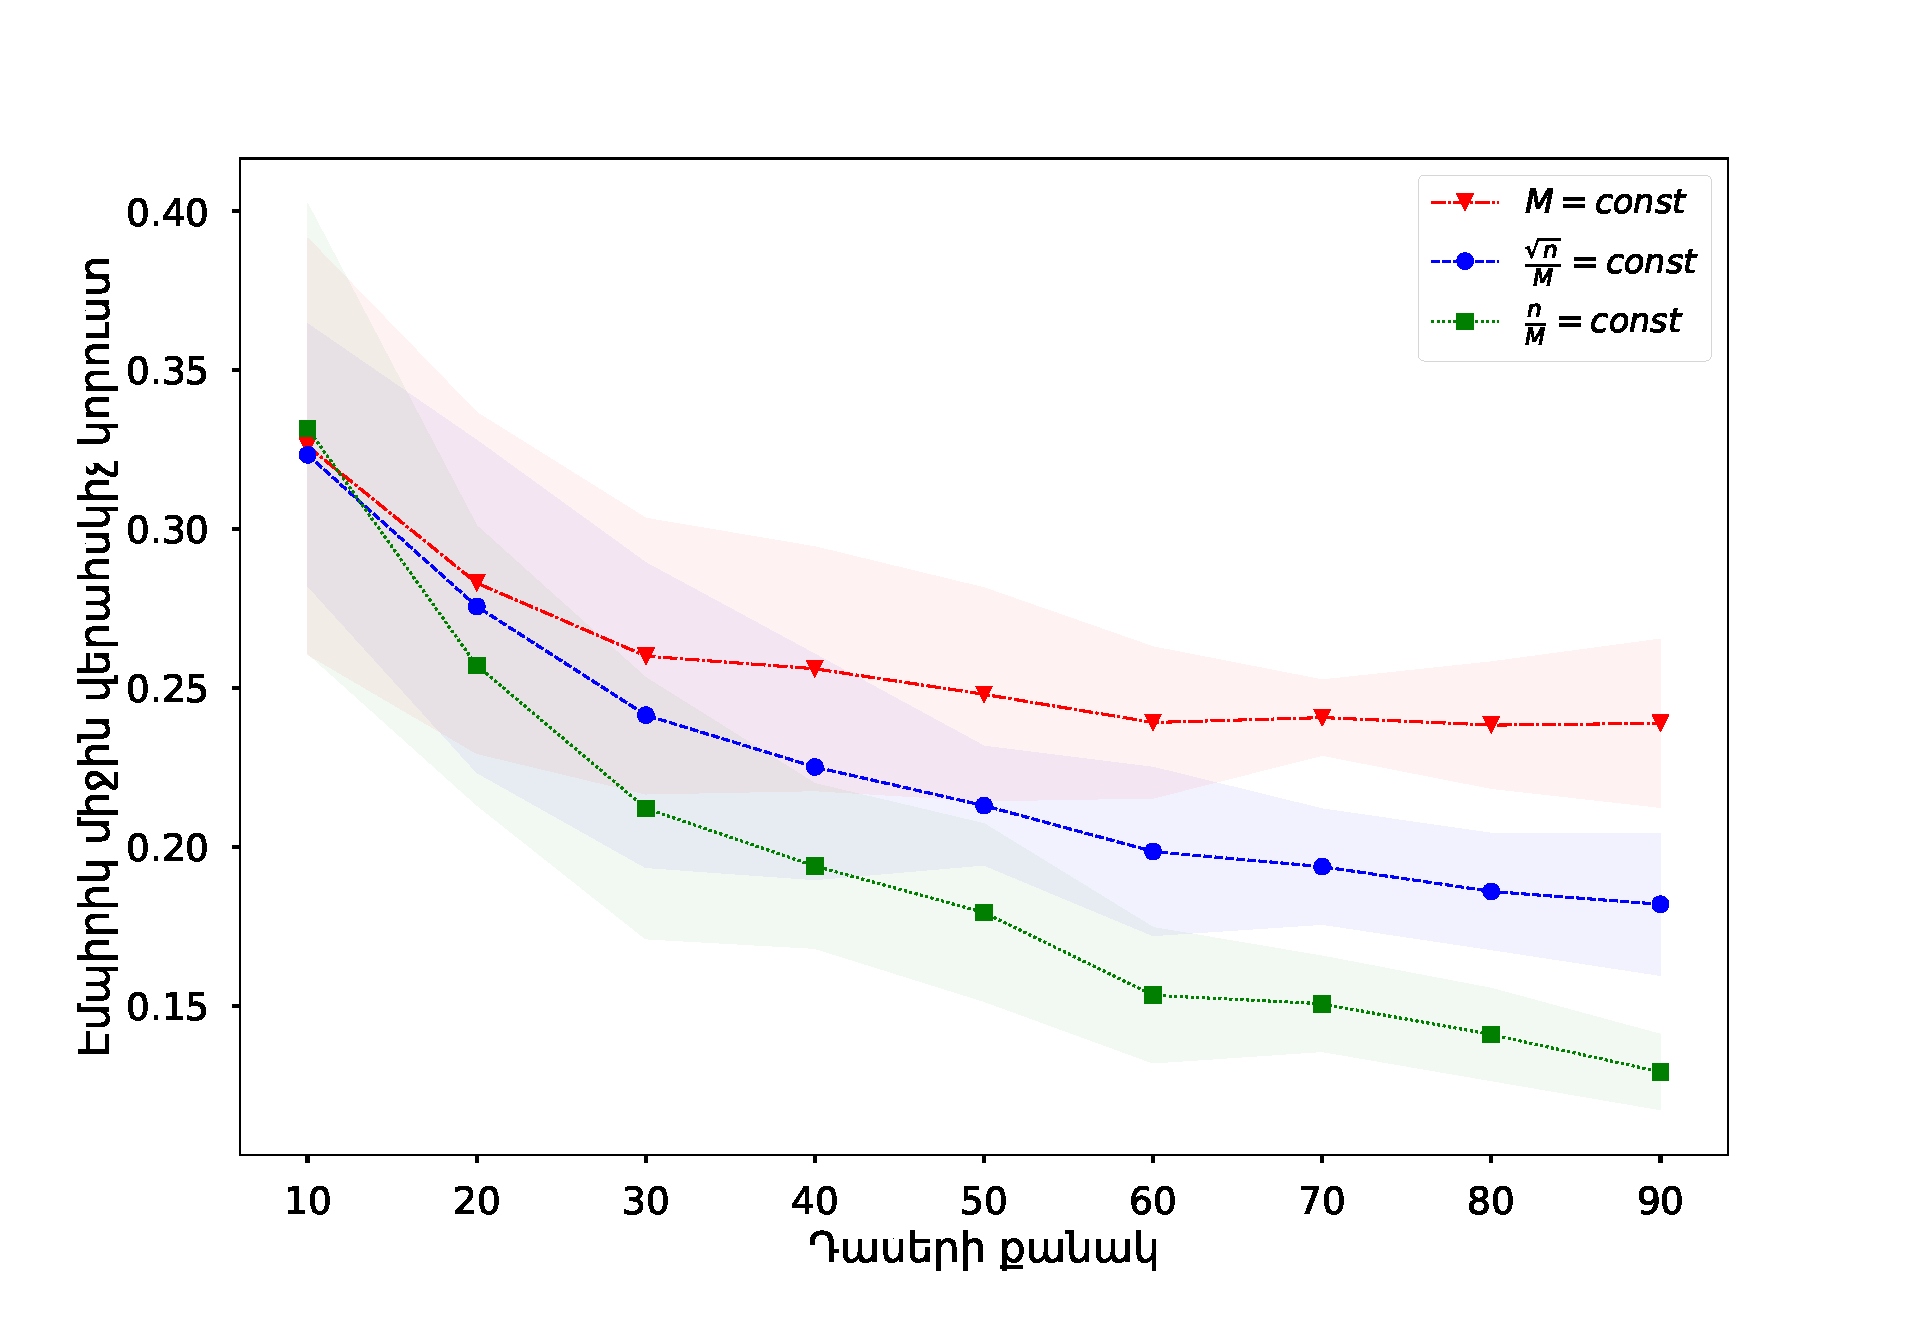
\includegraphics[width=.5\textwidth]{imgs/k=2.pdf}\hfill
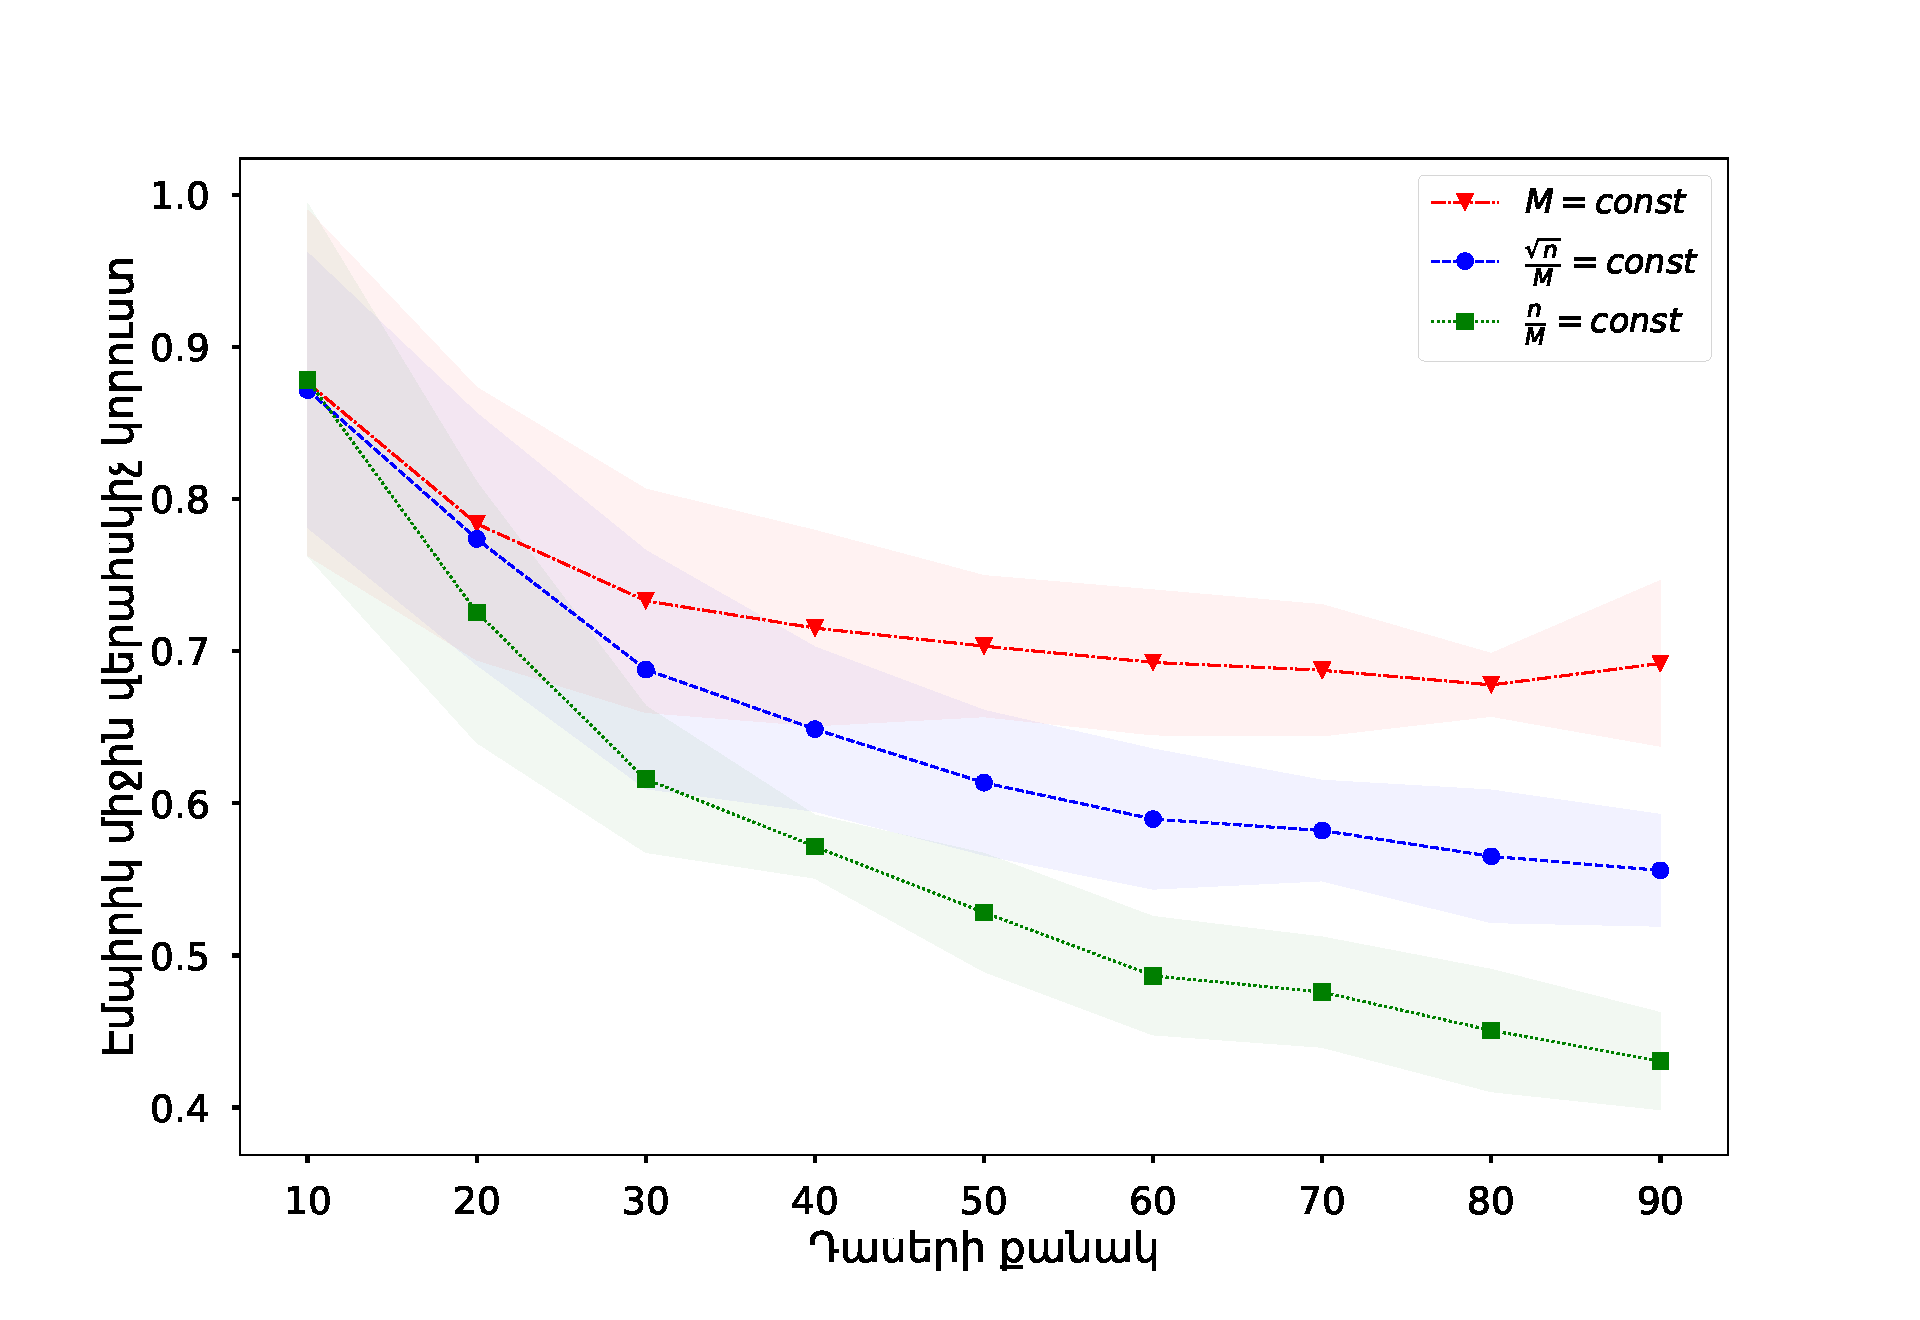
\includegraphics[width=.5\textwidth]{imgs/k=5.pdf}\hfill
\caption{\textit{Ձախ պատկերում $k=2$, իսկ աջում $k=5$  քանակությամբ դասերից բաղկացած առաջադրանքի էմպիրիկ միջին վերահսկիչ կորստի կախվածությունը՝ ներկայացումների ցանցի վարժեցման ժամանակ  օգտագործված դասերի քանակից։}}
\label{fig:figure3}

\end{figure}



\par Նեյրոնային ցանցի յուրաքանչյուր վարժեցումից հետո հեռացվում է վերջին շերտը, իսկ մնացած շերտերով  անցկացվում են նկարները, և նախավերջին շերտի ելքային արդյունքը համարվում է նկարի նոր ներկայացում։ 

\begin{figure}[htp]

\centering
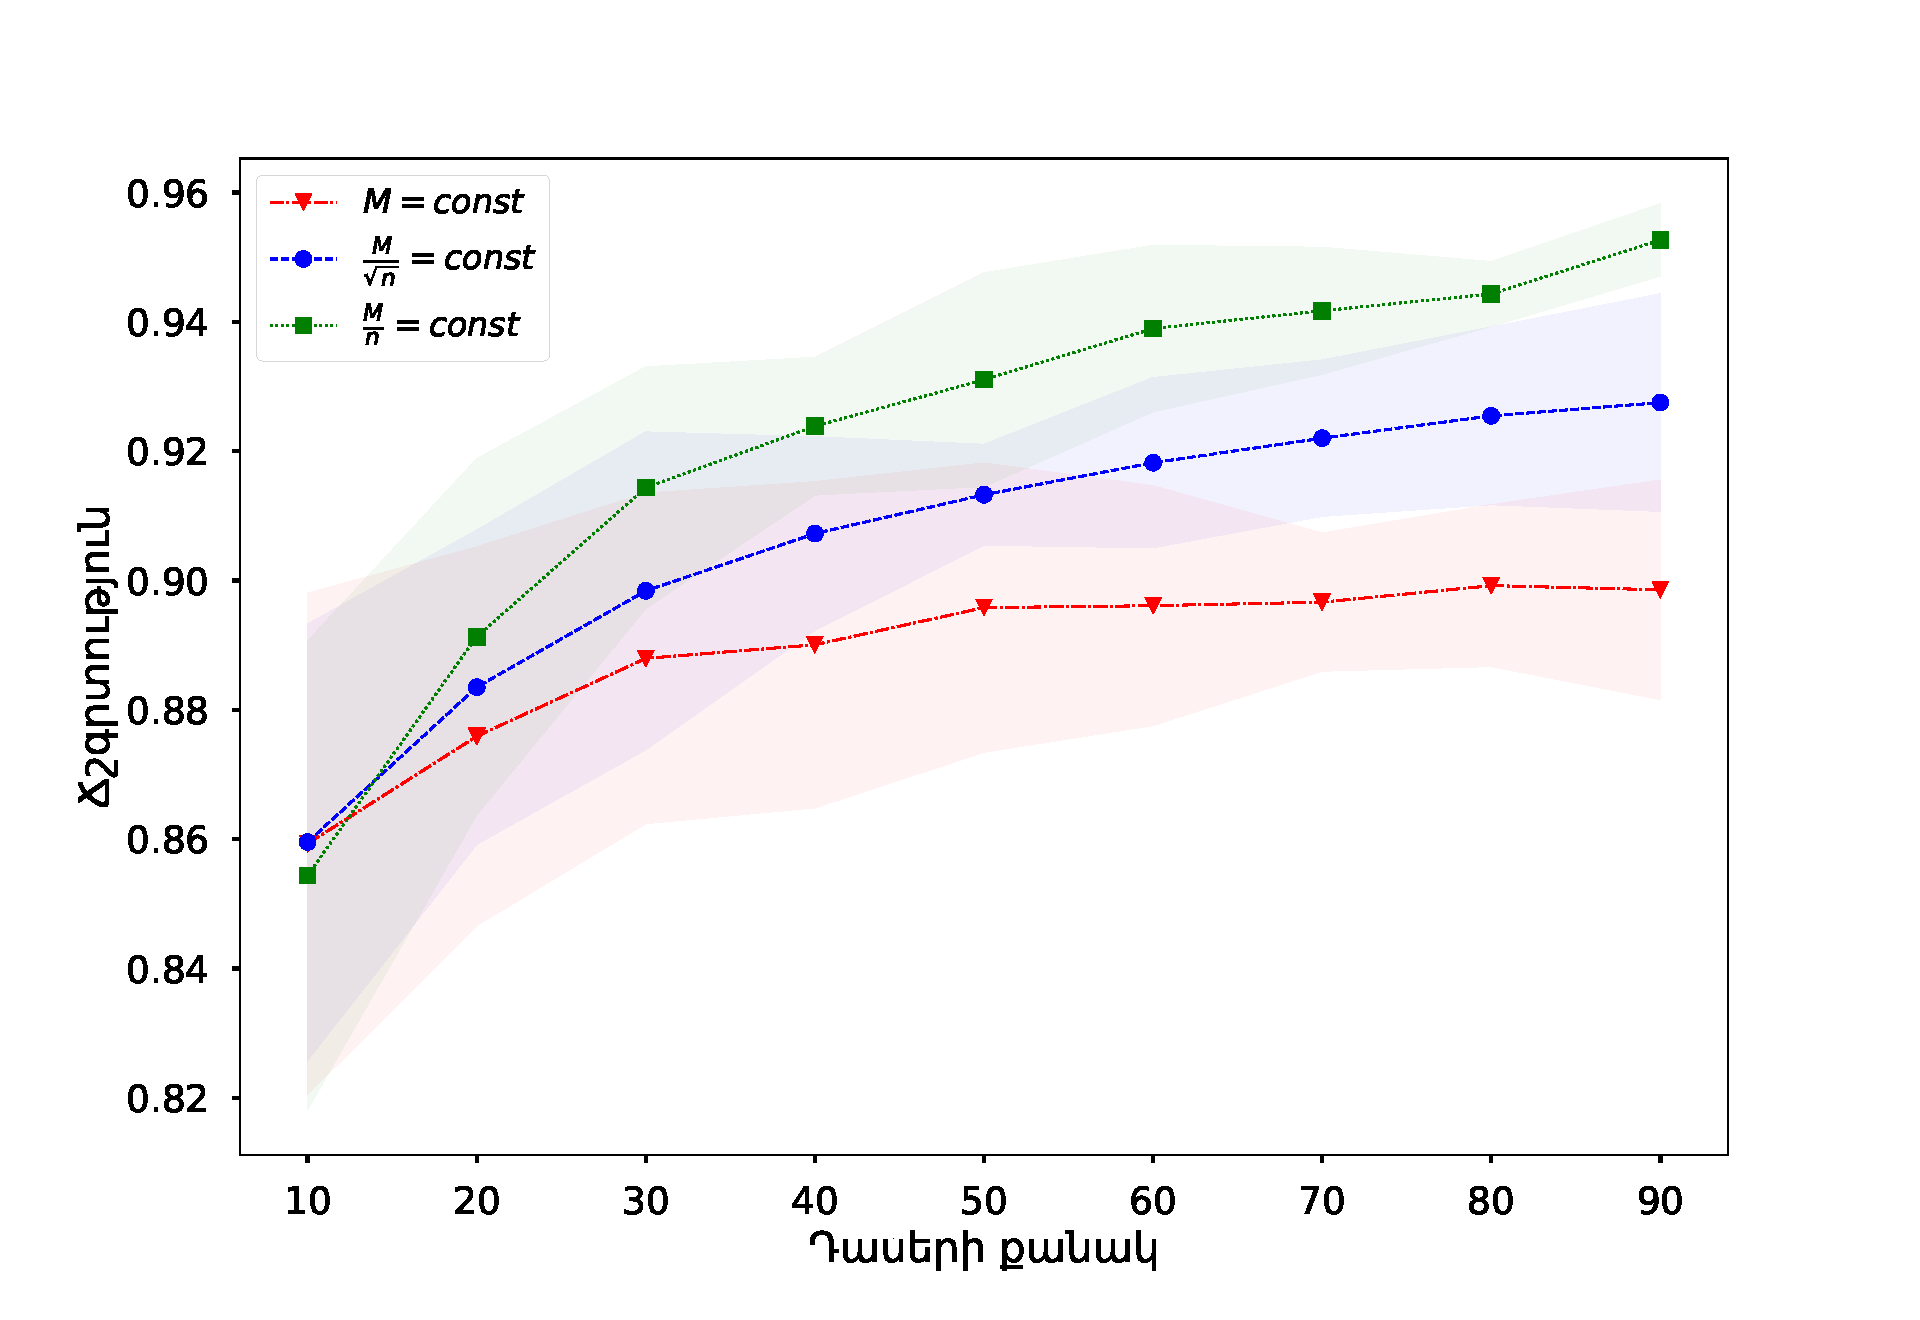
\includegraphics[width=.5\textwidth]{imgs/k=2_acc.pdf}\hfill
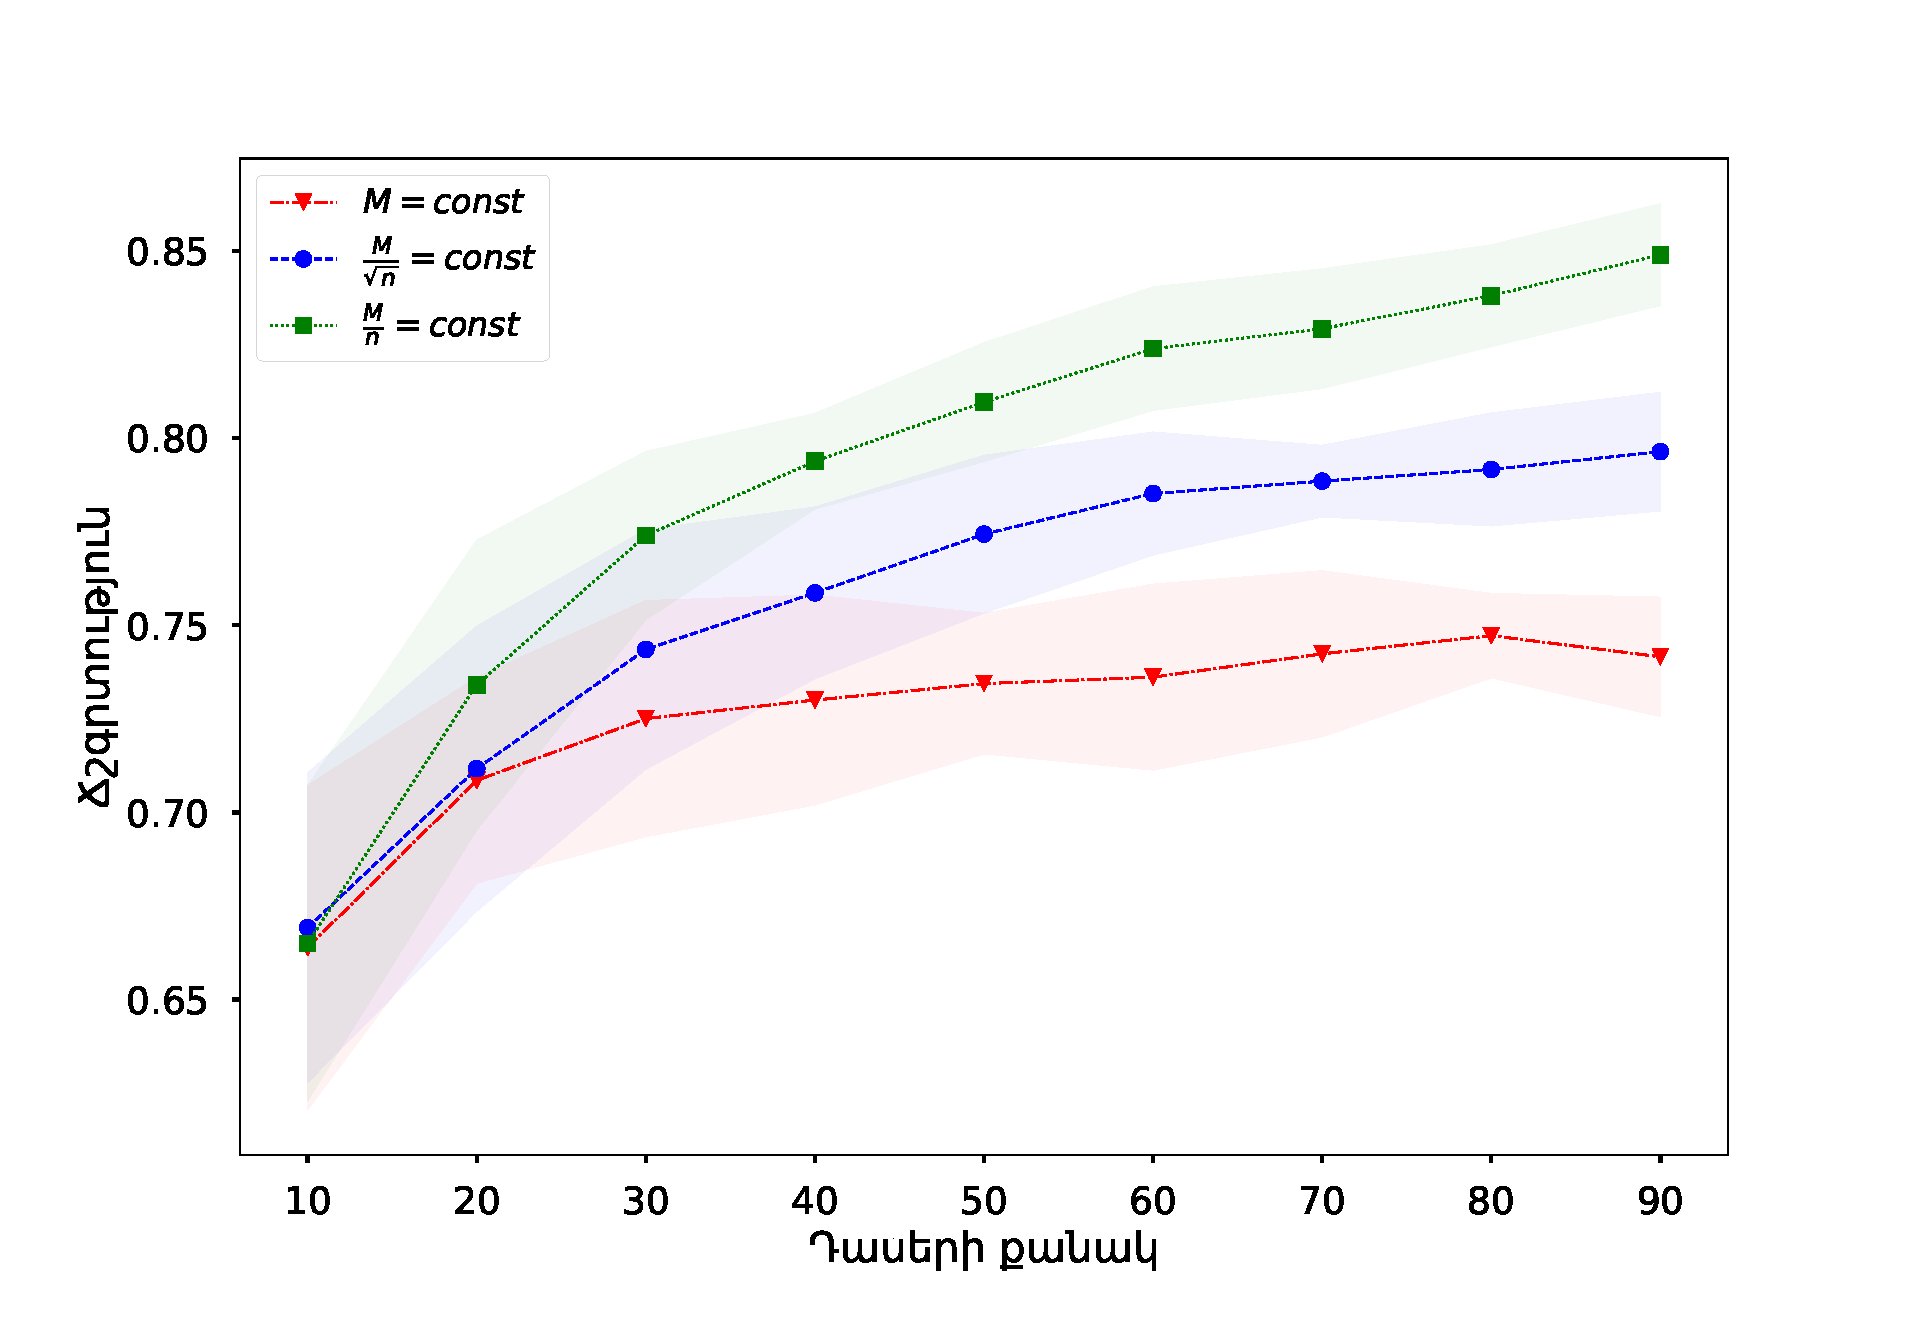
\includegraphics[width=.5\textwidth]{imgs/k=5_acc.pdf}\hfill
\caption{\textit{Ձախ պատկերում $k=2$, իսկ աջում $k=5$  քանակությամբ դասերից բաղկացած առաջադրանքի ճշգրտության կախվածությունը՝ ներկայացումների ցանցի վարժեցման ժամանակ  օգտագործված դասերի քանակից։}}
\label{fig:figure3}

\end{figure}

Մեր դիտարկած փաթույթային ցանցի նախավերջին շերտը պարունակում է $512$ նեյրոններ, ուստի նկարների ներկայացումների վեկտորի չափողականությունը նույնպես $512$ է։ Յուրաքանչյուր վարժեցված  ցանցի միջոցով ստացված նկարների ներկայացումների  վրա գծային դասակարգիչ է վարժեցվում ներկայացումներում չմասնակցող $k=2$, $k=5$ և $k=10$ քանակությամբ դասերից կազմված  առաջադրանքների համար։



\begin{figure}[htp]

\centering
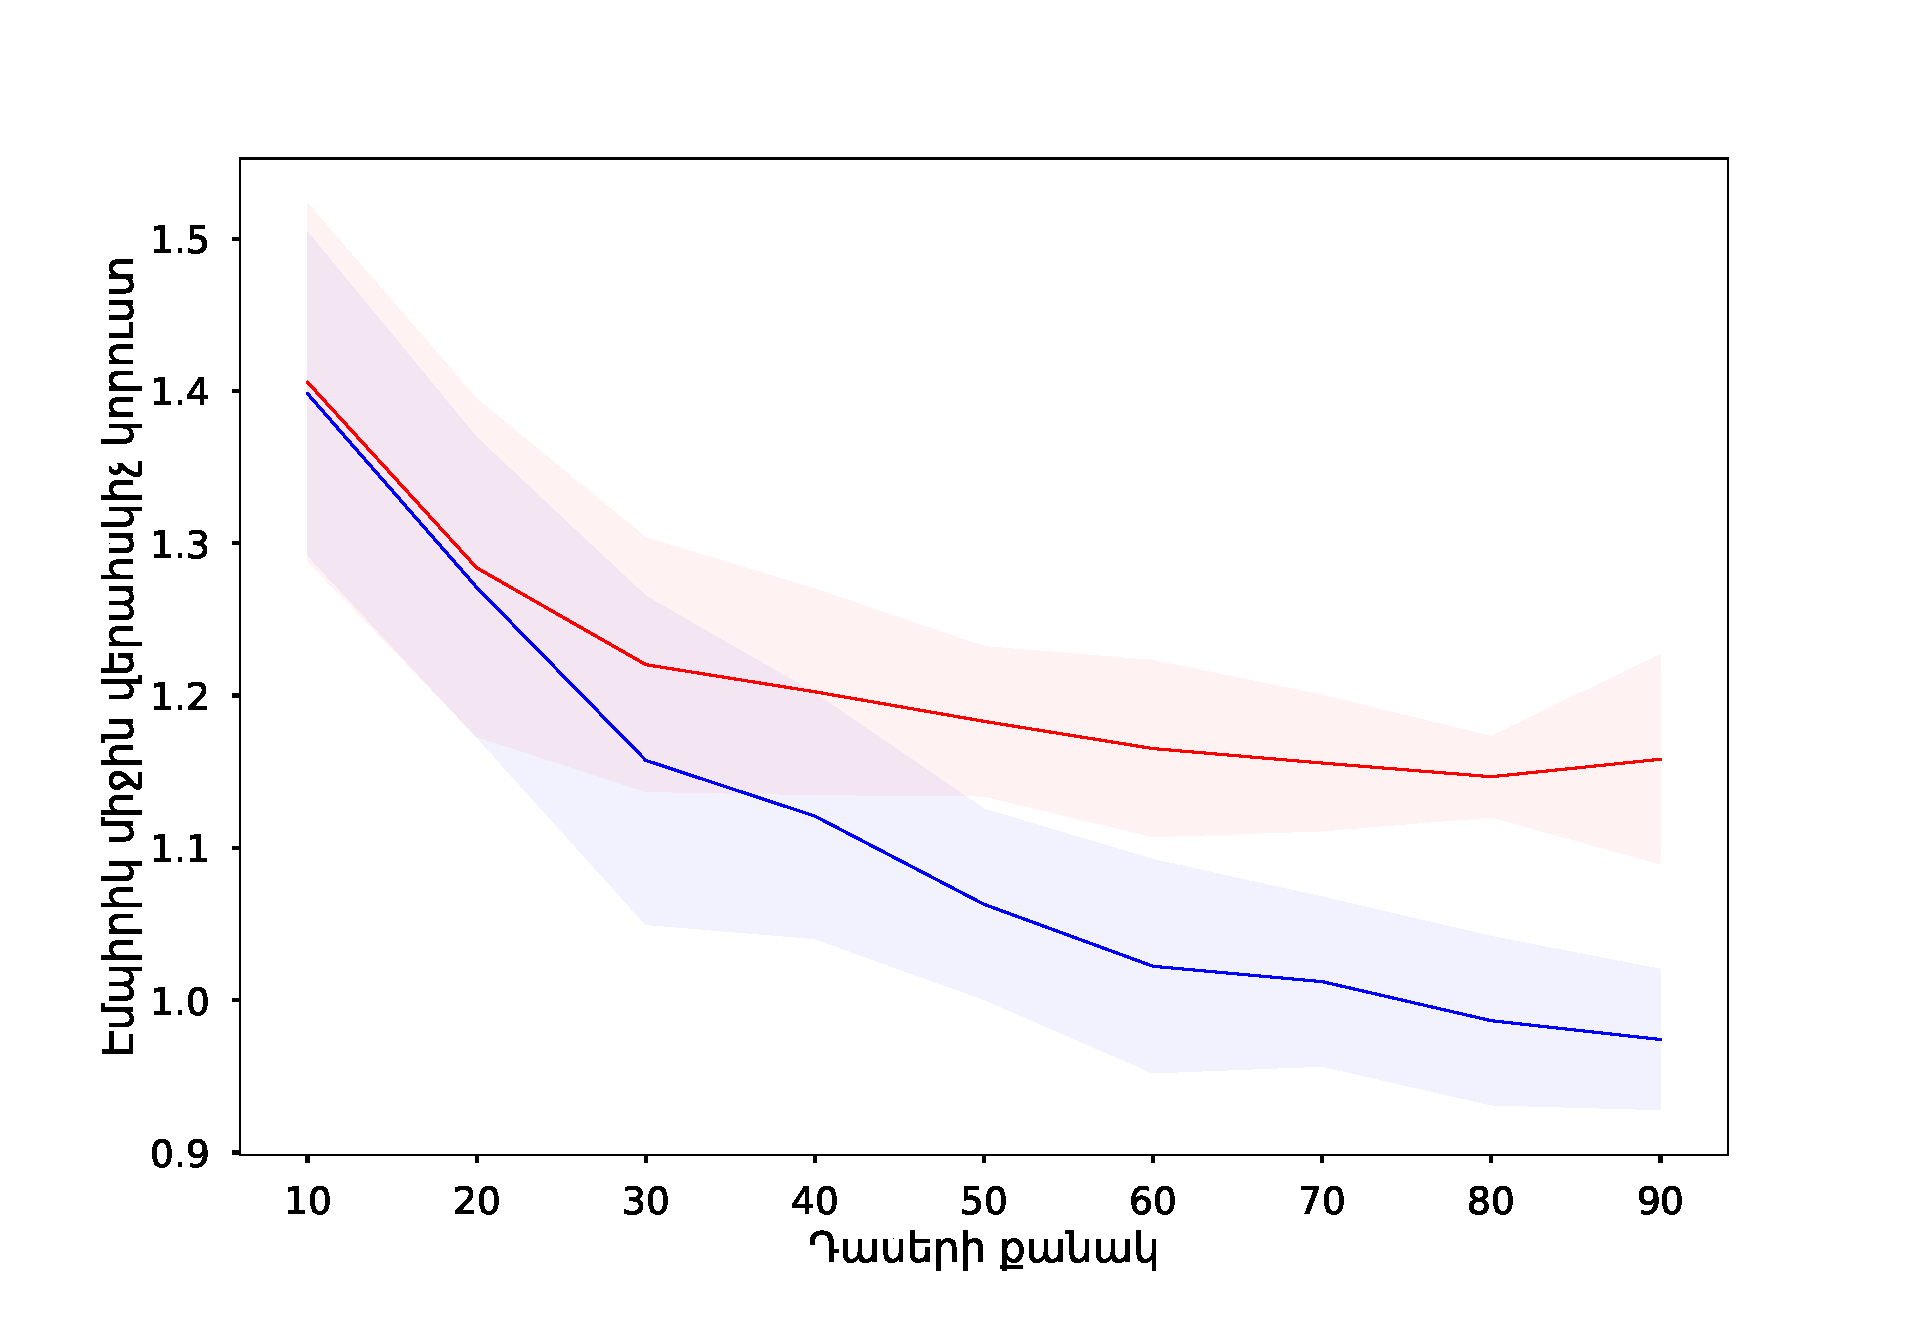
\includegraphics[width=.5\textwidth]{imgs/k=10.pdf}\hfill
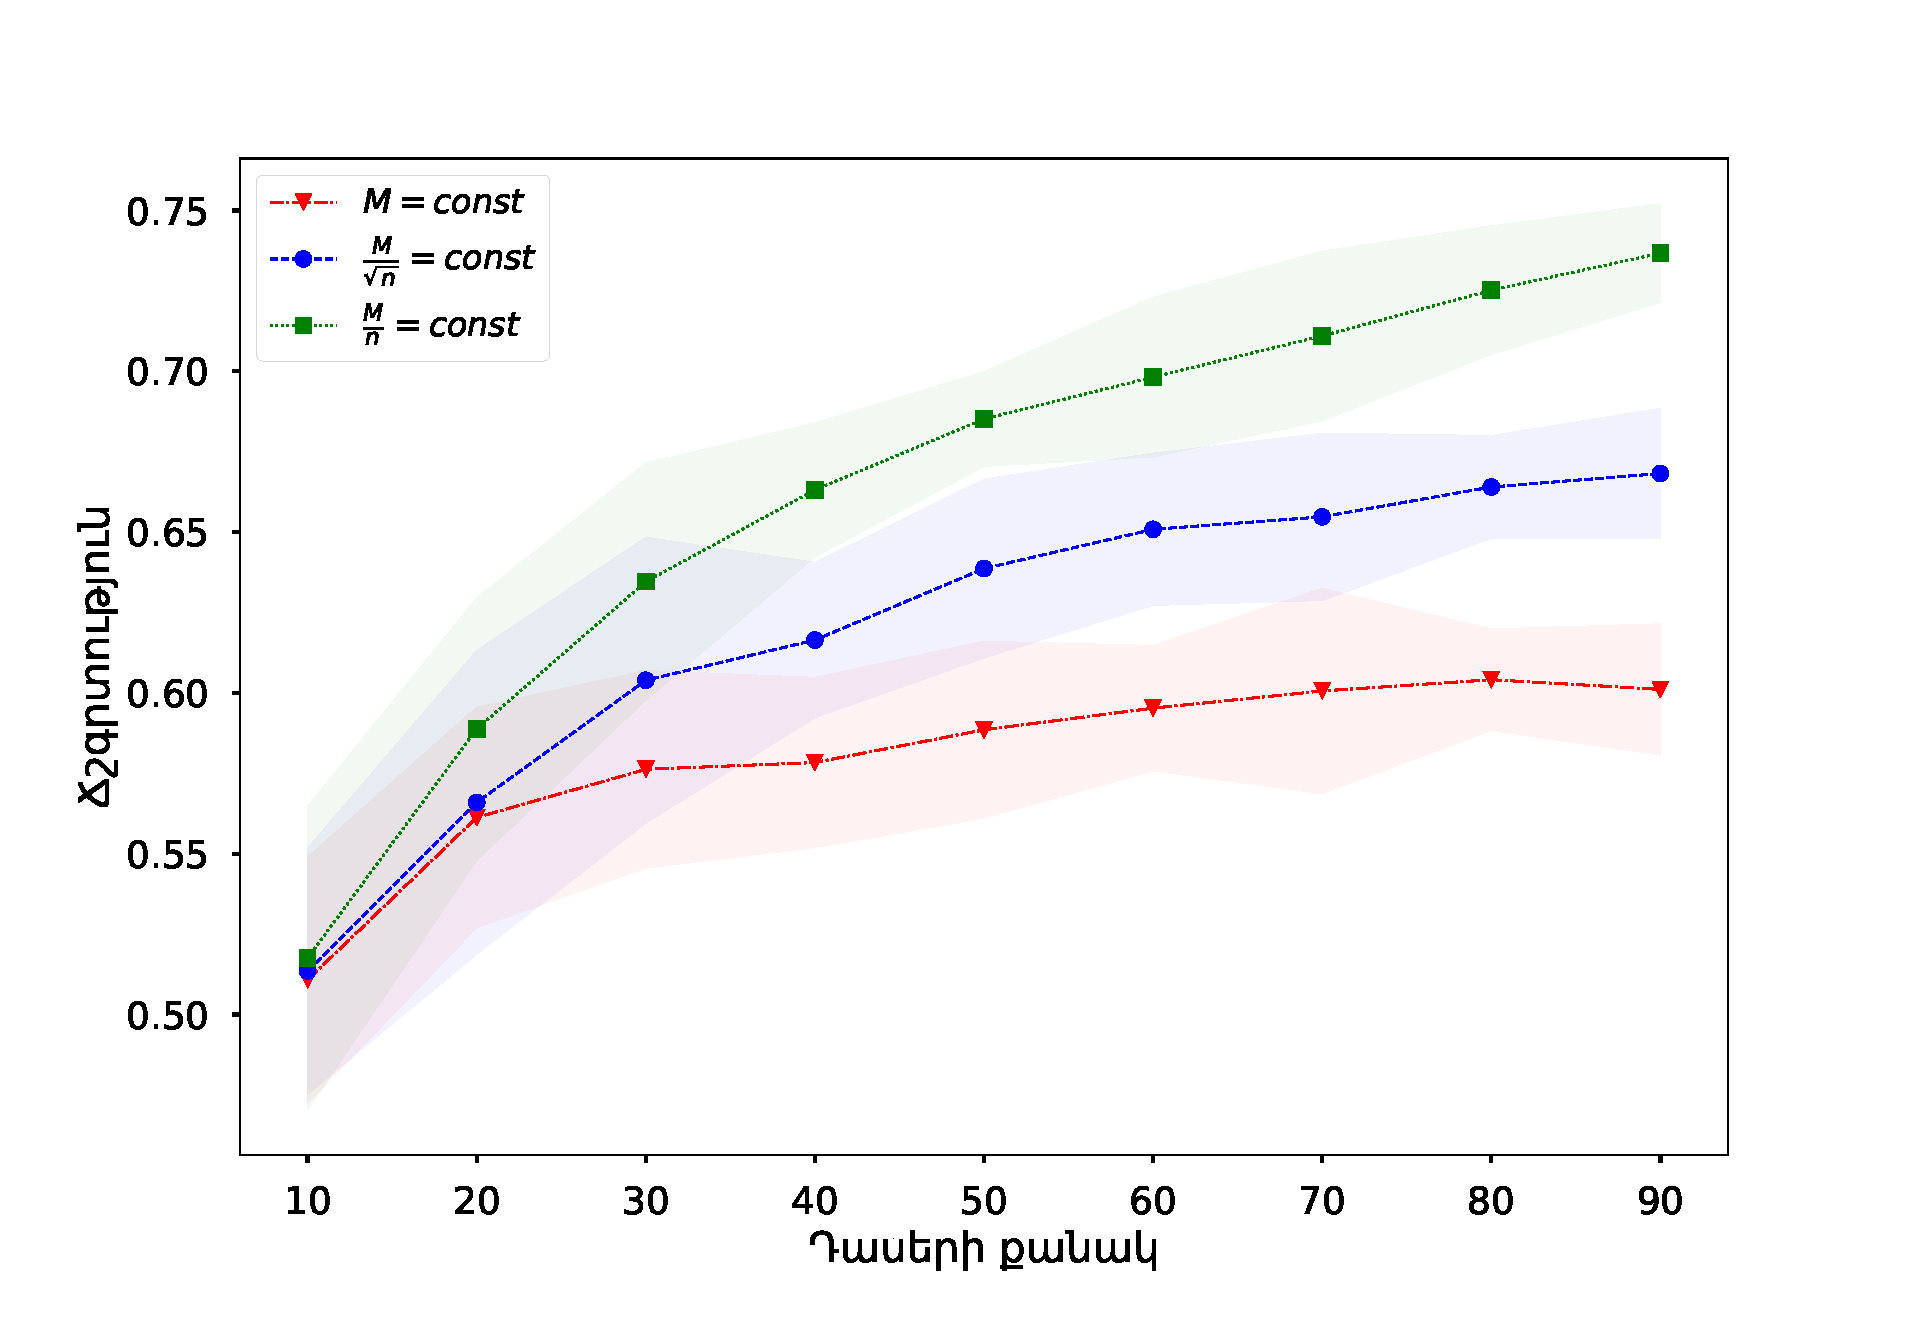
\includegraphics[width=.5\textwidth]{imgs/k=10_acc.pdf}\hfill
\caption{\textit{$k=10$ քանակությամբ դասերից բաղկացած առաջադրանքի ճշգրտության և էմպիրիկ միջին վերահսկիչ կորստի կախվածությունը՝ ներկայացումների ցանցի վարժեցման ժամանակ  օգտագործված դասերի քանակից։}}
\label{fig:figure3}

\end{figure}



\phantomsection
\addcontentsline{toc}{subsection}{Արդյունքները}


\subsection*{\hfill Արդյունքները \hfill} \noindent

\par Ինչպես վերահսկիչ միջին կորստի սխալանքի գնահատականում, այնպես էլ $CIFAR-100$ տվյալների բազմության վրա իրականացված փորձարկումների արդյունքում, պարզվում է, որ վերահսկվող առաջադրանքի ուսուցման միջոցով ստացվող նկարների ներկայացումները այլ առաջադրանքներում օգտագործելու դեպքում հասարակ գծային դասկարգչի բարձր ճշգրտությունը կամ ցածր կորուստը էապես կախված է դասերի քանակից՝ $n$-ից։  Երբ ուսուցման օրինակների քանակը պահում ենք հաստատուն՝ $M=5000$, բայց մեծացնում ենք դասերի քանակը՝ $n$-ը, ուսուցման մեջ չմասնակցող դասերից բաղկացած $k=2$, $k=5$, $k=10$ առաջադրանքների համապատասխանաբար $85.93$, $66.38$ և $51.07$ միջին ճշգրտությունները բարձանում են՝ դառնալով $89.85$, $74.15$ և $60.11$։ 
%
%\begin{figure}[htp]
%\centering
%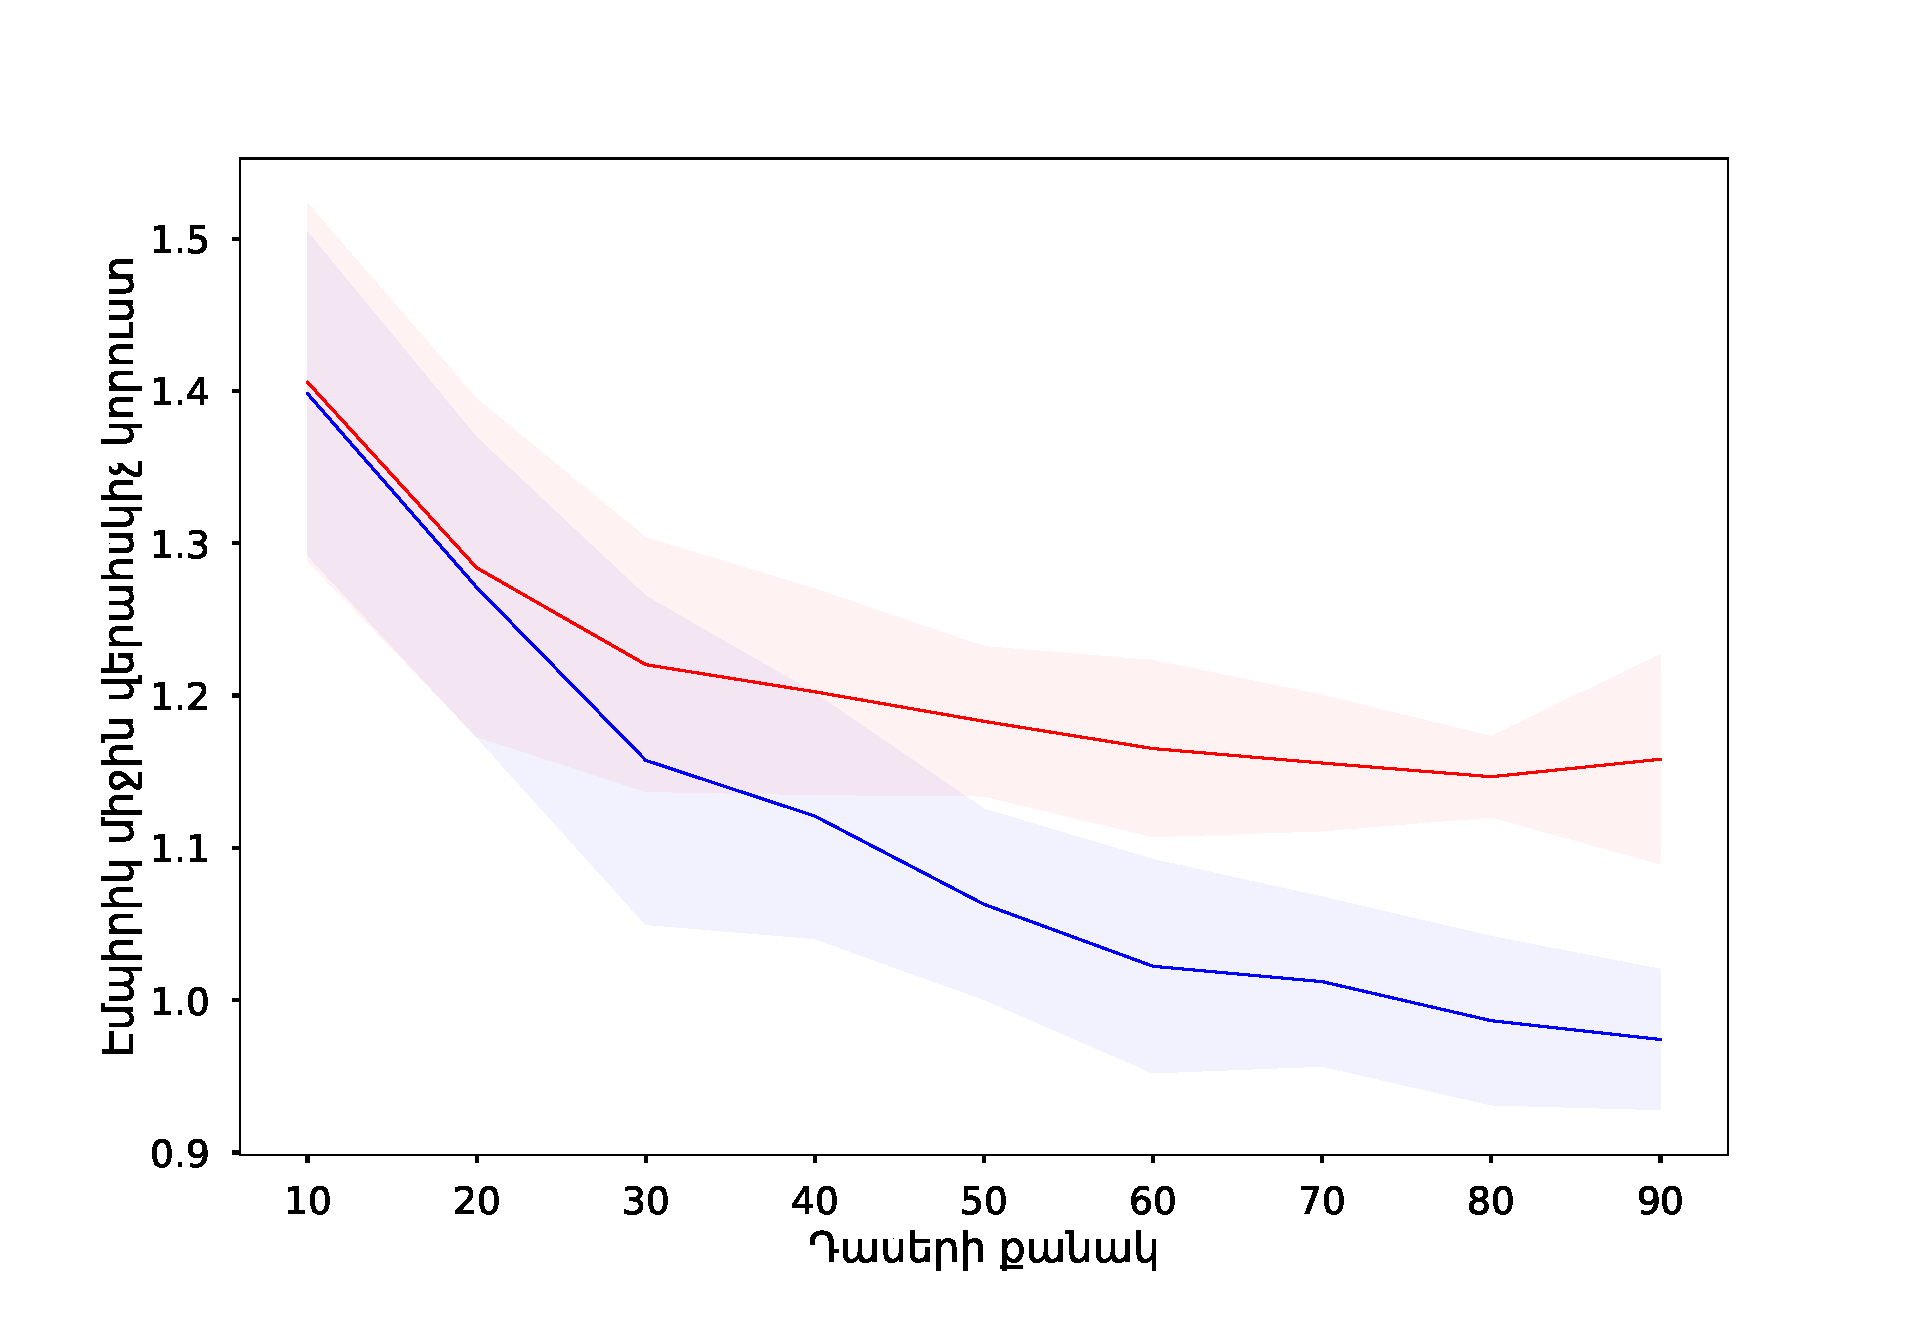
\includegraphics[width=1\textwidth]{imgs/k=10.pdf}\hfill
%\caption{\textit{$k=10$ քանակությամբ դասերից բաղկացած առաջադրանքի էմպիրիկ միջին վերահսկիչ կորստի կախվածությունը ներկայացումների ցանցի վարժեցման ժամանակ  օգտագործված դասերի քանակից։}}
%\label{fig:figure4}
%\end{figure}

\vspace{10mm}
%\begin{center}
%\begin{tabular}{|l|l|r|r|r|r|r|r|r|r|r|}
%\hline
%     & $n$ &    $n=10$ &    $n=20$ &    $n=30$ &    $n=40$ &    $n=50$ &    $n=60$ &    $n=70$ &    $n=80$ &    $n=90$ \\
%     \hline
%& $m$ &         &         &         &         &         &         &         &         &         \\
%\hline
% & $m=10$ & $1.406$ & $1.284$ & $1.220$ & $1.203$ & $1.183$ & $1.165$ & $1.156$ & $1.147$ & $1.158$ \\
%  $M=const$   & $2$ & $0.326$ & $0.283$ & $0.260$ & $0.256$ & $0.248$ & $0.239$ & $0.241$ & $0.238$ & $0.239$ \\
%     & $m=5$ & $0.877$ & $0.784$ & $0.733$ & $0.715$ & $0.703$ & $0.693$ & $0.687$ & $0.678$ & $0.692$ \\
%     \hline
% & $10$ & $1.403$ & $1.212$ & $1.067$ & $0.998$ & $0.938$ & $0.878$ & $0.854$ & $0.813$ & $0.785$ \\
%$\frac{M}{n} = const$     & $2$ & $0.332$ & $0.257$ & $0.212$ & $0.194$ & $0.179$ & $0.153$ & $0.151$ & $0.141$ & $0.129$ \\
%     & $5$ & $0.878$ & $0.726$ & $0.616$ & $0.571$ & $0.528$ & $0.487$ & $0.476$ & $0.451$ & $0.430$ \\
%     \hline
%  & $10$ & $1.398$ & $1.271$ & $1.158$ & $1.121$ & $1.063$ & $1.022$ & $1.012$ & $0.987$ & $0.974$ \\
% $\frac{M}{\sqrt{n}} = const$    & $2$ & $0.323$ & $0.276$ & $0.241$ & $0.225$ & $0.213$ & $0.199$ & $0.194$ & $0.186$ & $0.182$ \\
%     & $5$ & $0.872$ & $0.774$ & $0.688$ & $0.649$ & $0.614$ & $0.590$ & $0.582$ & $0.565$ & $0.556$ \\
%\hline
%\end{tabular}
%\end{center}



%\begin{tabular}{|l||r|r|r||r|r|r||r|r|r||}
% \cline{2-10}
%  \multicolumn{1}{c|}{} & \multicolumn{3}{|l||}{\hspace{10mm} $M=const$} & \multicolumn{3}{|l||}{\hspace{10mm} $\frac{M}{\sqrt{n}} = const$ } & \multicolumn{3}{|l||}{$\hspace{10mm} \frac{M}{n} = const$} \\
% \cline{2-10}
%  \multicolumn{1}{c|}{} &     $k=2$ &     $k=5$ &     $k=10$ &    $k=2$ &     $k=5$ &     $k=10$ &    $k=2$ &     $k=5$ &     $k=10$ \\
%\hline
%$n=10$                & $0.326$ & $0.877$ & $1.406$ & $0.323$ & $0.872$ & $1.398$ & $0.332$ & $0.878$ & $1.403$ \\
%\hline
%$n=20$                & $0.283$ & $0.784$ & $1.284$ & $0.276$ & $0.774$ & $1.271$ & $0.257$ & $0.726$ & $1.212$ \\
%\hline
%$n=30$                & $0.260$ & $0.733$ & $1.220$ & $0.241$ & $0.688$ & $1.158$ & $0.212$ & $0.616$ & $1.067$ \\
%\hline
%$n=40$                & $0.256$ & $0.715$ & $1.203$ & $0.225$ & $0.649$ & $1.121$ & $0.194$ & $0.571$ & $0.998$ \\
%\hline
%$n=50$                & $0.248$ & $0.703$ & $1.183$ & $0.213$ & $0.614$ & $1.063$ & $0.179$ & $0.528$ & $0.938$ \\
%\hline
%$n=60$                & $0.239$ & $0.693$ & $1.165$ & $0.199$ & $0.590$ & $1.022$ & $0.153$ & $0.487$ & $0.878$ \\
%\hline
%$n=70$                & $0.241$ & $0.687$ & $1.156$ & $0.194$ & $0.582$ & $1.012$ & $0.151$ & $0.476$ & $0.854$ \\
%\hline
%$n=80$                & $0.238$ & $0.678$ & $1.147$ & $0.186$ & $0.565$ & $0.987$ & $0.141$ & $0.451$ & $0.813$ \\
%\hline
%$n=90$                & $0.239$ & $0.692$ & $1.158$ & $0.182$ & $0.556$ & $0.974$ & $0.129$ & $0.430$ & $0.785$ \\
%\hline
%\end{tabular}


\begin{center}
\captionof{table}{\textit{$M=const$, $\frac{M}{\sqrt{n}} = const$ և $\frac{M}{n} = const$ դեպքերում միջին գծային դասակարգչի ճշգրտությունների կախվածությունը $n$-ից և $k$-ից։}}
\vspace{2mm}
\begin{tabular}{|l||r|r|r||r|r|r||r|r|r||}
 \cline{2-10}
  \multicolumn{1}{c|}{} & \multicolumn{3}{|l||}{\hspace{10mm} $M=const$} & \multicolumn{3}{|l||}{\hspace{10mm} $\frac{M}{\sqrt{n}} = const$ } & \multicolumn{3}{|l||}{$\hspace{10mm} \frac{M}{n} = const$} \\
 \cline{2-10}
  \multicolumn{1}{c|}{} &     $k=2$ &     $k=5$ &     $k=10$ &    $k=2$ &     $k=5$ &     $k=10$ &    $k=2$ &     $k=5$ &     $k=10$ \\
\hline
$n=10$                  & $85.930$ & $66.386$ & $51.077$ & $85.955$ & $66.918$ & $51.352$ & $85.440$ & $66.498$ & $51.760$ \\
\hline
$n=20$                 & $87.590$ & $70.856$ & $56.126$ & $88.350$ & $71.168$ & $56.594$ & $89.130$ & $73.404$ & $58.875$ \\
\hline
$n=30$                 & $88.795$ & $72.506$ & $57.624$ & $89.840$ & $74.356$ & $60.393$ & $91.435$ & $77.400$ & $63.458$ \\
\hline
$n=40$                 & $89.005$ & $73.002$ & $57.835$ & $90.725$ & $75.866$ & $61.643$ & $92.385$ & $79.386$ & $66.309$ \\
\hline
$n=50$                 & $89.580$ & $73.442$ & $58.853$ & $91.325$ & $77.436$ & $63.865$ & $93.105$ & $80.966$ & $68.515$ \\
\hline
$n=60$                 & $89.610$ & $73.614$ & $59.526$ & $91.820$ & $78.522$ & $65.085$ & $93.895$ & $82.396$ & $69.817$ \\
\hline
$n=70$                 & $89.665$ & $74.238$ & $60.060$ & $92.200$ & $78.854$ & $65.473$ & $94.170$ & $82.928$ & $71.096$ \\
\hline
$n=80$                 & $89.920$ & $74.724$ & $60.410$ & $92.545$ & $79.166$ & $66.401$ & $94.430$ & $83.810$ & $72.518$ \\
\hline
$n=90$                 & $89.855$ & $74.156$ & $60.107$ & $92.750$ & $79.642$ & $66.821$ & $95.265$ & $84.906$ & $73.671$ \\
\hline
\end{tabular}
\end{center}
\vspace{3mm}
\par Այժմ ուշադիր ուսումնասիրենք միջին ճշգրտությունների աղյուսակը։ Երբ  $\frac{M}{n}=const$ և $n=30$, ապա ուսուցման օրինակների քանակը հավասար է $\frac{M}{\sqrt{n}}=const$ և $n=90$ դեպքի ուսուցման օրիկնարի քանակին։ $k=2, k=5$ և $k=10$ քանակությամբ դասերից բաղկացած առաջադրանքների $\frac{M}{n}=const$ և $n=30$  դեպքի համապատասխանաբար $91.43$, $77.40$ և $63.45$ ճշգրտությունները բարձրանում  են  $\frac{M}{\sqrt{n}}=const$ և $n=90$ ժամանակ՝ դառնալով $92.75$, $79.64$ և $66.82$։


\pagebreak

\section*{\hfill Եզրակացություն \hfill} \noindent
\phantomsection
\addcontentsline{toc}{section}{Եզրակացություն}


\par Այս աշխատանքում տեսականորեն հիմնավորվեց վերահսկվող առաջադրանքի ուսուցմամբ ստացվող ներկայացումների միջոցով իրականացվող տրանսֆերային ուսուցման մեթոդը, որը լայն կիրառություններ ունի այնպիսի խնդիրների տիրույթներում, որտեղ սահմանափակ քանակությամբ պիտակավորված տվյալներ կան։ Դուրս բերվեց միջին վերահսկիչ կորստի սխալանքի գնահատական, որտեղ ներակայացումների ուսուցման առաջադրանքում մասնակցող դասերի քանակը մեծ ազդեցություն ունի այլ առաջադրանքներում ընդհանրացման ժամանակ։ $CIFAR-100$ տվյալների վրա իրականցված փորձարկումները նույնպես հաստատեցին, որ դասերի մեծ քանակը կարևոր է  առավել պիտանելի և նոր առաջադրանքներում ընդհանրացվող ներկայացումներ սովորելու համար։
\par Հետագա աշխատանքները ուղղված կլինեն այլ տվյալների բազմության վրա՝ աշխատանքում իրականացված նմանատիպ փորձարկումների միջոցով, ներկայացումների առաջադրանքում մասնակցող դասերի քանակի և էմպիրիկ միջին վերահսկիչ կորստի կախվածության հետազոտմանը։

Աշխատանքում իրակացված փորձարկումների ծրագիրը հասանելի է հետևյալ հասցեով՝ \url{https://github.com/Gevorg-Minasyan/fine-tune-tj}։
  
\pagebreak
\medskip
\begin{thebibliography}{9}
\phantomsection
\addcontentsline{toc}{section}{Գրականություն} 

\bibitem{bib_item_12}
S. Arora, H. Khandeparkar, M. Khodak, O. Plevrakis and N. Saunshin.
\textit{ A Theoretical Analysis of Contrastive Unsupervised Representation Learning.} https://arxiv.org/abs/1902.09229, 2019.

\bibitem{bib_item_1}
S. Pan and Q. Yang.
\textit{A survey on transfer learning.}  Knowledge and Data Engineering, IEEE Transactions on,
22(10):1345–1359, 2010.

\bibitem{bib_item_2}
K. Weiss, T. M. Khoshgoftaar, and D. Wang. \textit{ A survey of transfer learning.} 
Journal of Big Data, vol. 9, no. 3, 2016.

\bibitem{bib_item_3}
C. Tan, F. Sun, T. Kong, W. Zhang, C. Yang, and C. Liu.
\textit{A survey on deep transfer learning.}  https://arxiv.org/abs/1808.01974, 2018.

\bibitem{bib_item_19}
M. E. Peters, M. Neumann, M. Iyyer, M. Gardner, C. Clark, K. Lee, and L. Zettlemoyer. \textit{Deep contextualized word representations.} NAACL, 2018.

\bibitem{bib_item_6}
Devlin, J., Chang, M.-W., Lee, K., and Toutanova. \textit{K. Bert: Pretraining of deep bidirectional transformers for language understanding.} arXiv preprint arXiv:1810.04805, 2018.


\bibitem{bib_item_7}
Logeswaran, L. and Lee, H. \textit{An efficient framework for
learning sentence representations.}  In Proceedings of the
International Conference on Learning Representations,
2018.

\bibitem{bib_item_15}
A. Krizhevsky, I. Sutskever and G. Hinton.\textit{ Imagenet classification with deep convolutional
neural networks.} In Advances in neural information processing systems, pp. 1097–1105, 2012.

\bibitem{bib_item_4}
K. Simonyan and A. Zisserman. \textit{ Very deep convolutional networks
for large-scale image recognition.} In ICLR, 2015


\bibitem{bib_item_16}
C. Szegedy, W. Liu, Y. Jia, P. Sermanet, S. Reed, D. Anguelov, D. Erhan, V. Vanhoucke, and A. Rabinovich. \textit{Going deeper with convolutions.} In CVPR, 2015.

\bibitem{bib_item_5}
K. He, X. Zhang, S. Ren, and J. Sun. \textit{Deep
residual learning for image recognition.} In
Proceedings of CVPR, pages 770–778, 2016.
arxiv.org/abs/1512.03385

\bibitem{bib_item_18}
Tomas Mikolov, Kai Chen, Greg Corrado, and Jeffrey Dean. \textit{Efficient estimation of word representations
in vector space.} ICLR Workshop, 2013.

\bibitem{bib_item_17}
J. Pennington, R. Socher, and C. D. Manning. \textit{GloVe: Global vectors for word representation.} In EMNLP, 2014.

\bibitem{bib_item_8}
A. Razavian, H. Azizpour, J. Sullivan, and S. Carlsson. \textit{ CNN Features off-the-shelf: an Astounding Baseline
for Recognition.} CoRR, abs/1403.6382, 2014.

\bibitem{bib_item_9}
M.  Mohri, A. Rostamizadeh and A. Talwalkar.  \textit{Foundations of Machine Learning.} MIT press, 2018.

\bibitem{bib_item_10}
Shai Shalev-Shwartz and Shai Ben-David. \textit{Understanding Machine Learning: From Theory to Algorithms.} Cambridge University Press, New York, NY, USA, 2014.

\bibitem{bib_item_11}
A. Maurer. \textit{A vector-contraction inequality for rademacher
complexities.} In International Conference on Algorithmic Learning Theory, pp. 3–17. Springer, 2016.

\bibitem{bib_item_13}
J.V. Burke. \textit{Nonlinear Optimization.} 
University of Washington, 2004.

\bibitem{bib_item_14}
A. Krizhevsky.  \textit{Learning multiple layers of features from
tiny images.} Technical report, 2009.

\end{thebibliography}

\end{document}
